
\chapter[Ontological Structures to Personalize the Gamification in CL Scenarios]{Ontological Structures to Personalize the Gamification in Collaborative Learning Scenarios}
\label{chapter:ontogacles-1}

This chapter presents the formalization of ontological structures that have been proposed by the author of this thesis dissertation to represent gamified CL scenarios. These ontological structures allow us to systematically represent knowledge extracted from player types models and needs-based theories of motivation to deal with the motivation problem caused by the scripted collaboration. This knowledge corresponds to concepts identified by the author of this thesis as relevant to solve the context-dependency related to the individual user characteristics, so that the ontological structures described in this chapter are also used to represent ontological models to personalize the gamification in CL scenarios based on player types models and need-based theories of motivation. The ontological structures to represent gamified CL scenarios have been developed as an extension of ontological structures proposed to represent CL scenarios in the CL ontology, hence the chapter starts with an overview of the CL ontology (\autoref{sec:overview-of-cl-ontology}). The ontological structures that have been formalized in the \emph{\textbf{Onto}logy to \textbf{Ga}mify \textbf{C}ollaborative \textbf{Le}arning \textbf{S}cenarios} - \textbf{OntoGaCLeS} to represent gamified CL scenarios based on the knowledge extracted from player types models and needs-based theories of motivation are presented in \autoref{sec:modeling-gamified-cl-scenarios}. To demonstrate the usefulness of this formalization, and then to validate the ontological structures as a formal representation of ontological models to personalize the gamification in CL scenarios, \autoref{sec:formalizing-ontological-model} shows the procedure followed to build an ontological model to personalize the gamification of CL scenarios based on the Dodecad player type models \cite{Marczewski2015b}. Finally, \autoref{sec:ontogacles1-concluding-remarks} presents the concluding remarks of this chapter.

Part of the work described in this chapter was published by the author of this PhD thesis dissertation in the scientific articles:

\begin{itemize}
\item
\aspas{\emph{Towards an Ontology for Gamifying Collaborative Learning Scenarios}} published in the 12\textsuperscript{th} International Conference on Intelligent Tutoring Systems, ITS 2014, held in Honolulu, HI, USA \cite{ChallcoMoreiraMizoguchiIsotani2014a}.

\item
\aspas{\emph{An Ontology Engineering Approach to Gamify Collaborative Learning Scenarios}} published in the 20\textsuperscript{th} International Conference on Collaboration and Technology, CRIWG 2014, held in Santiago, Chile \cite{ChallcoMoreiraMizoguchiIsotani2014}.

\item
\aspas{\emph{Personalization of Gamification in Collaborative Learning Contexts using Ontologies}} published as Volume 13, Issue 6, in the journal of IEEE Latin America Transactions, 2015 \cite{ChallcoMoreiraBittencourtMizoguchiIsotani2015}.
\end{itemize}

%%%%%%%%%%%%%%%%%%%%%%%%%%%%%%%%%%%%%%%%%%%%%%%%%%%%

\section{Overview of the Collaborative Learning Ontology}
\label{sec:overview-of-cl-ontology}

The CL ontology has been developed for a long time by the contributions of many researchers. Initially, the CL ontology was conceived to support the opportunistic group formation \cite{IkedaGoMizoguchi1997}, so that, to identify situations in which an individual shifting from individual learning mode to CL mode, the CL ontology has been formalized the agreement in the negotiation process for group formation as ontological structures that describe individual and group learning goals. Employing this formalization, intelligent agents have been developed to help students to find group members for establishing group learning activities in which they should participate. These agents check the individual and group learning goals, and then they initiate a negotiation process to establish an agreement of whom participate in group learning activities. This first version of the CL ontology has been demonstrated to be useful in the development of agent-based systems that provide helpful support for the group formation \cite{InabaOhkuboIkedaMizoguchiToyoda2001, SupnithiInabaIkedaMizoguchi1999}.

In order to provide theoretical and pedagogical justification for the group formation, the first version of the CL ontology has been extended to represent CL scenario that compliant with instructional and learning theories \cite{InabaMizoguchi2004,IsotaniMizoguchiIsotaniCapeliIsotanideAlbuquerqueBittencourtJaques2013}. In this extension, concepts, such as interaction patterns, group goals, individual goals, CL roles and so on, have been formalized from different instructional/learning theories, so that, in addition to support the group formation \cite{IsotaniMizoguchi2008}, the ontological structures to represent CL scenarios have been successfully applied in: the modeling of learners' development \cite{InabaIkedaMizoguchi2003} the interaction analysis \cite{InabaOhkuboIkedaMizoguchi2002}, and the design of CL process \cite{IsotaniMizoguchiIsotaniCapeliIsotanideAlbuquerqueBittencourtJaques2013}.

\autoref{fig:concepts-terms-and-relation-in-cl-ontology} shows the terms, concepts and relations defined in the CL ontology. These concepts are defined as follows as:

\begin{description}
 \item[\textbf{I-goal}] is the individual learning goal that represents what the participant in focus (\emph{I}) is expected to acquire, and it is described as a change in his/her learning stage.

 \item[\textbf{I-role}] is the CL role played by the participant in focus (\emph{I}).

 \item[\textbf{You-role}] is the CL role played by the participant (\emph{You}) who is interacting with the participant in focus (\emph{I}).

 \item[\textbf{Y<=I-goal}] is the learning strategy employed by the participant in focus (\emph{I}) to interact with the participant (\emph{You}) in order to achieve his/her individual learning goals (\emph{I-goal}).

 \item[\textbf{W(L)-goal}] is the common learning goal for the group members in the CL scenario.

 \item[\textbf{W(A)-goal}] is the rational arrangement of the group activity used to achieve the common learning goal (\emph{W(L)-goal}) and the individual learning goals (\emph{I-goal}).
\end{description}

\begin{figure}[!htb]
 \caption{Concepts, terms and relations defined in the CL Ontology}
 \label{fig:concepts-terms-and-relation-in-cl-ontology}
 \centering
 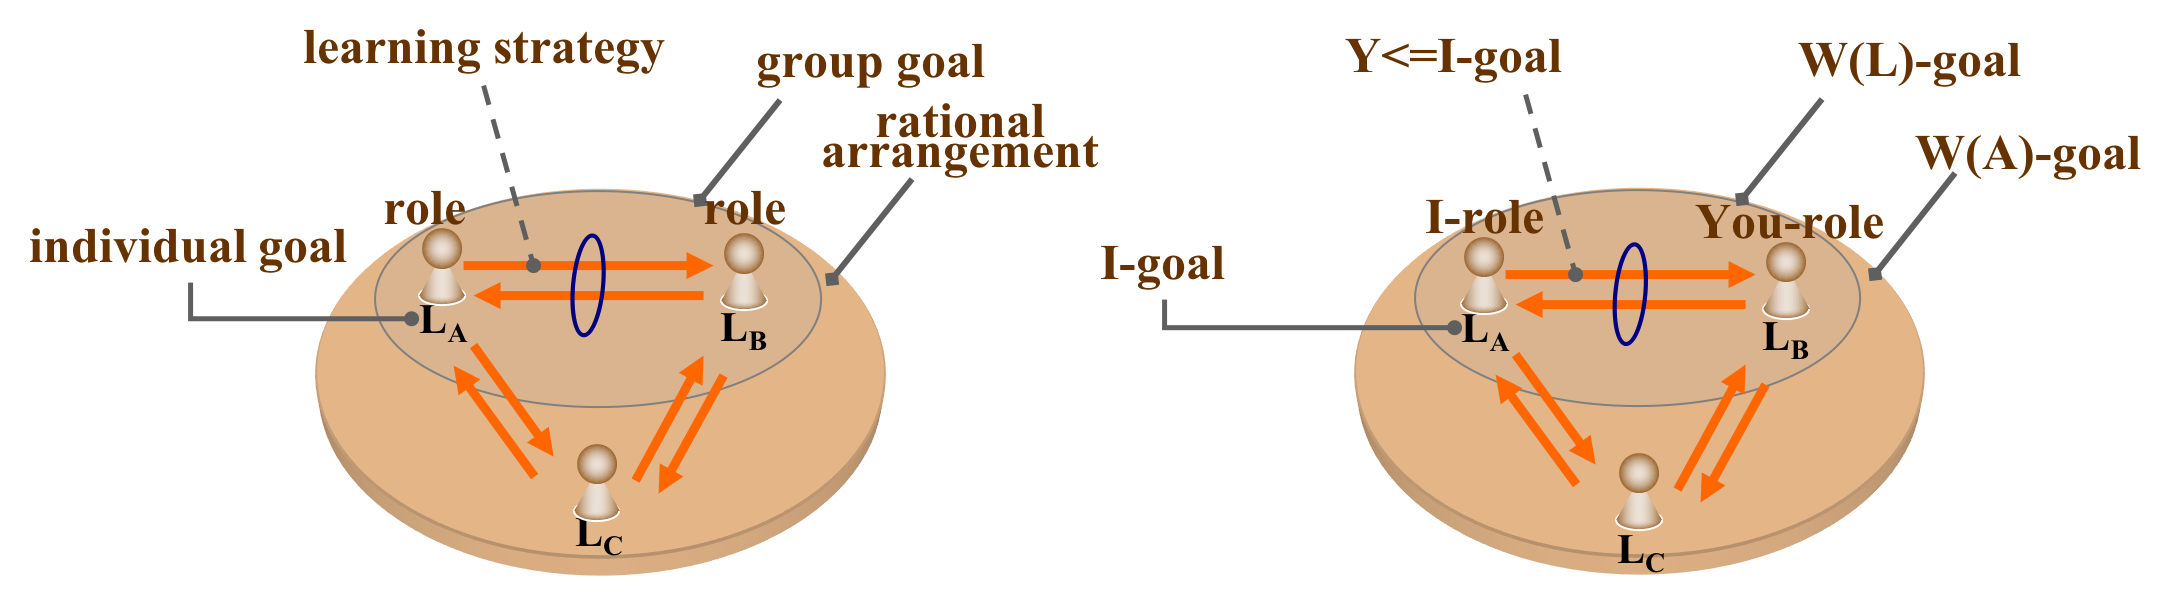
\includegraphics[width=0.95\textwidth]{images/chap-ontogacles1/concepts-terms-and-relation-in-cl-ontology.png}
 \fdireta{Isotani2009}
\end{figure}

To express the relationship of concepts described above, the CL Ontology employs the ontological structures shown in \autoref{fig:ontological-structure-cl-scenario} to represent CL scenarios. In these ontological structures, a CL scenario is represented by three parts defined as:  the \emph{Group structure benefit} (\emph{W(S)-goal}) to describe the expected benefits of the structured collaboration (i.e. positive interdependence, individual accountability, promotive interactions); the \emph{Learning strategy} (\emph{Y<=I-goal}) to describe the learning strategies employed by the group members in the CL scenario; and (3) the \emph{CL process} to describe the rational arrangement of the group activity (\emph{W(A)-goal}).

\begin{figure}[!htb]
 \caption{Ontological structure to represent CL scenarios}
 \label{fig:ontological-structure-cl-scenario}
 \centering
 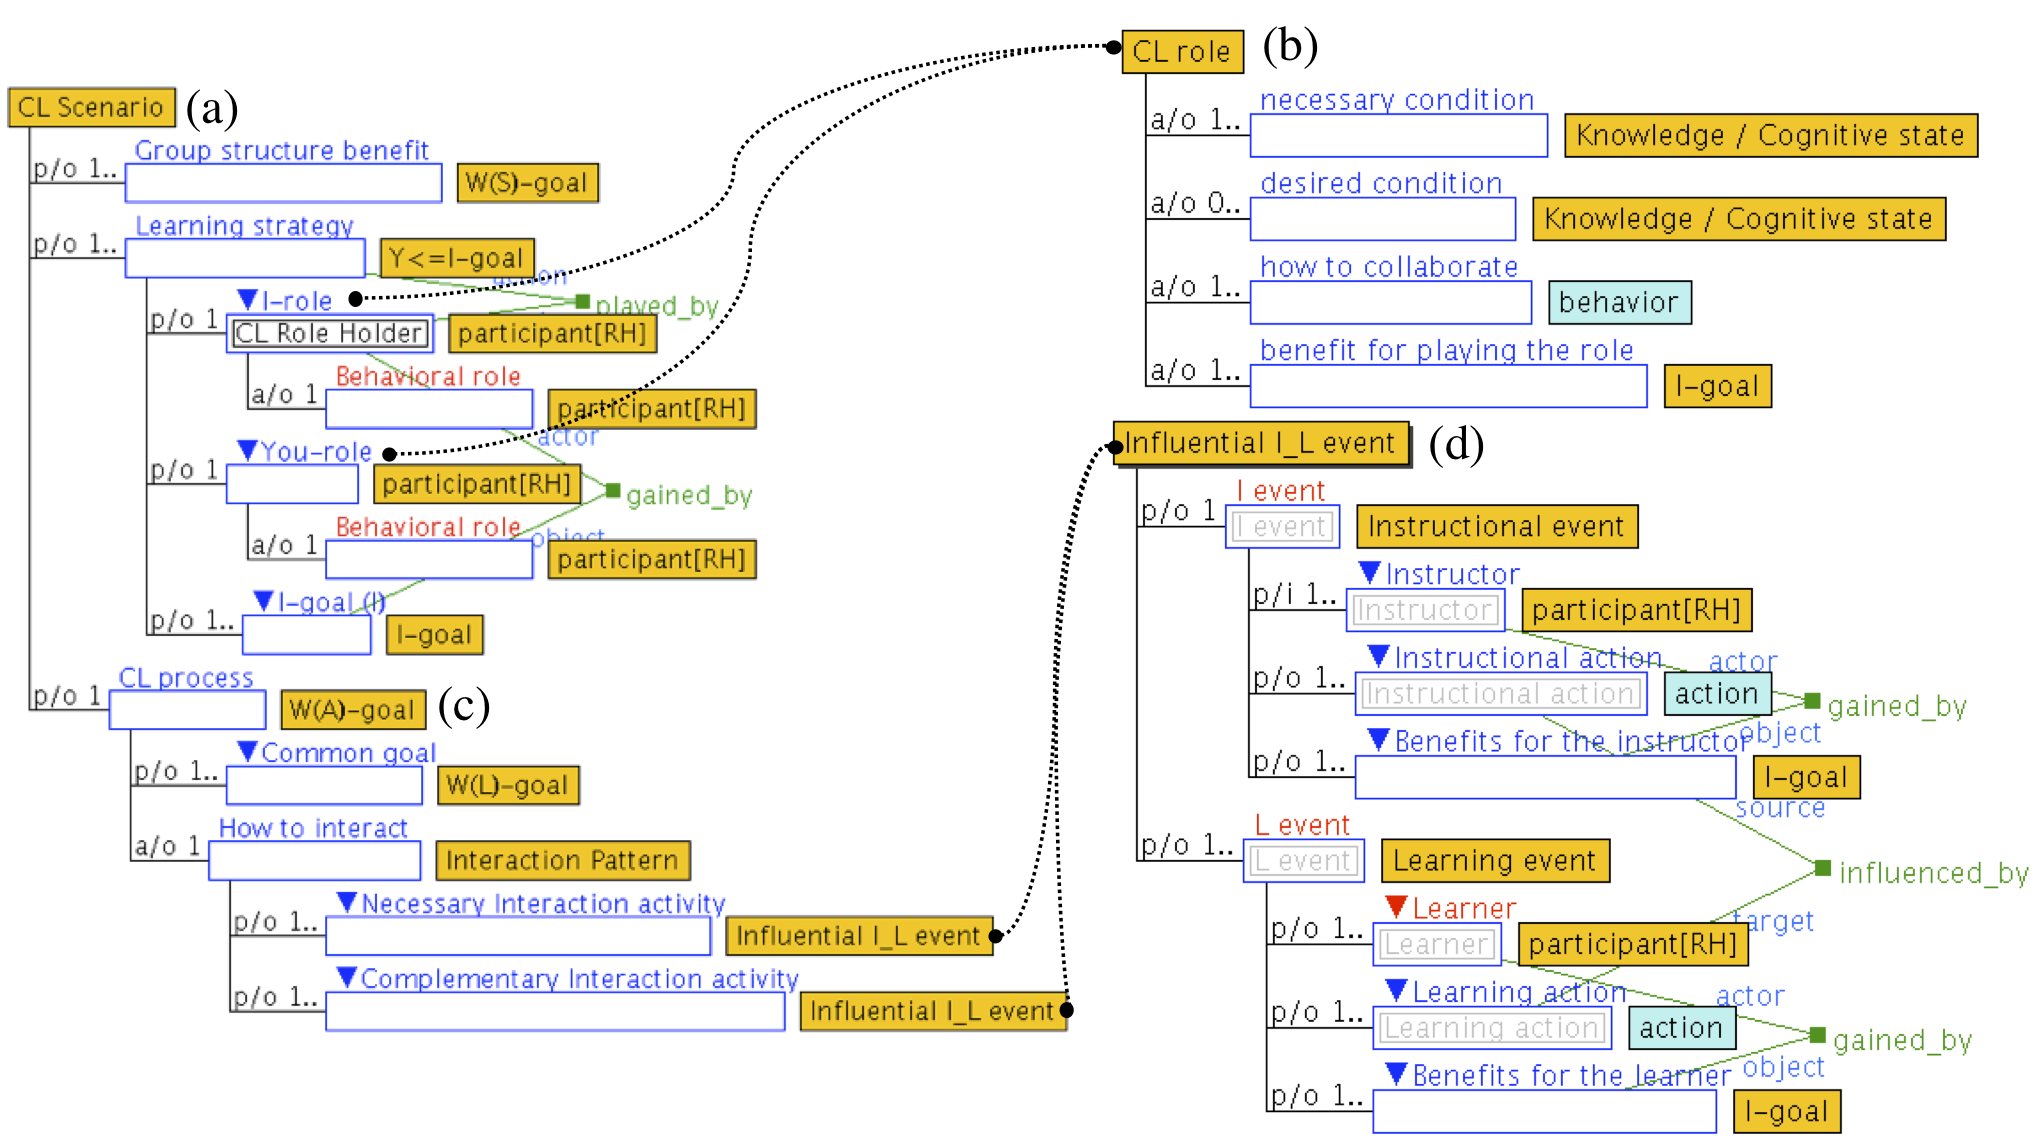
\includegraphics[width=1\textwidth]{images/chap-ontogacles1/ontological-structure-cl-scenario.png}
 \fdireta{Isotani2009}
\end{figure}

\begin{enumerate} [label=(\alph*)]

\item
The \textbf{Learning strategies} (\emph{Y<=I-goal}) are guidelines that specify how the participants should interact with others members of group to achieve their individual goals. These guidelines help the group members to externalize a desired behavior to play a given CL role more adequately. Therefore, the Learning strategy is represented as an ontological structure composes by: the participant in focus (\emph{I}) who plays the CL role \aspas{\emph{I-role}}, the participant (\emph{You}) who interacts with the participant in focus (\emph{I}) playing the CL role \aspas{\emph{You-role},} and the individual learning goals (\emph{I-goal}) that are expected to be achieved by the participant in focus (\emph{I}) at the end of CL scenario. The \emph{behavioral role} as part of the CL roles \aspas{\emph{I-role}} and \aspas{\emph{You-role}} is used to describe the behaviors externalized by the participants \aspas{\emph{I}} and \aspas{\emph{You}} when they interact in the CL scenario employing the learning strategy (\emph{Y<=I-goal}).

\item
The \textbf{CL role} describes functions, goals, duties and responsibilities that must be taken by members of group to achieve the common and individual learning goals. Thus, the ontological structure to represent a CL role is composed by: the \emph{necessary condition} and \emph{desired conditions} to play the CL role, the description of \emph{how to collaborate} when a group member plays the CL role, and the description of \emph{benefits for playing the role}. In this ontological structure, \emph{Cognitive/Knowledges states} are used to define the necessary and desired conditions for a group member to play the CL role, \emph{behaviors} are used to describe \emph{how to collaborate} playing the CL role, and individual learning goals (\emph{I-goal}) are employed to describe the expected \emph{benefits for playing the role}.

\item
The \textbf{CL process} is the \emph{rational arrangement of group activity} (\emph{W(A)-goal}) whereby the common and individual learning goals are achieved by the group members. This arrangement is represented by the \emph{common learning goals} (\emph{W(L)-goal}) as result of the negotiation process in the group formation, and by the \emph{Interaction Pattern} as the sequencing mechanism followed by the participants to achieve their individual learning goals (\emph{I-goal}). The interaction pattern is represented as a set of \emph{necessary} and \emph{desired interactions} in which the interaction for the group members is described as influential Instructional-Learning events (\emph{Influential I\_L events}).

\item
The \textbf{Influential I\_L event} represents the interaction among the group members and the benefits obtained by the interaction from two viewpoints: from the viewpoint of participants who play a role of instructor, and from the viewpoint of participants who play a role of learner. The influential I\_L event describes group members performing actions that influence other members with the purpose to change their own learning states by helping others to achieve their individual learning goals. Therefore, the ontological structure to represent an influential I\_L event is composed by two events: a \emph{learning event} and an \emph{instructional event} in which the participants are represented as actors of CL scenario playing CL roles and performing a set of actions to achieve their individual learning goals (\emph{I-goal}). For a group member acting as \emph{instructor}, the influential I\_L event describes his/her interaction with other group member who acts as \emph{learner} by means of instructional actions, and the expected \emph{benefits for the instructor} (\emph{I-goal}). For a group member acting as \emph{learner}, the influential I\_L event describes his/her interaction with other group member who acts as \emph{instructor} by means of learning actions, and the expected \emph{benefits for the learner} (\emph{I-goal}).
\end{enumerate}

As it was said before, the ontological structures shown in \autoref{fig:ontological-structure-cl-scenario} are used to describe CL scenarios that compliant with instructional and learning theories. To illustrate this, \autoref{fig:cognitive-apprenticeship-ontological-structure} shows the representation of a CL scenario based on the Cognitive Apprentice theory. According to this theory, the CL activities should incorporate situations that are familiar to those who are using these activities, and these situations must to lead the participants to act and interact acquiring skills in a specific context, and then generalizing these skills to other situations. Therefore, the CL scenarios based on the Cognitive Apprentice theory focuses on supporting a more skilled participant (known as \emph{master}) to teach a familiar situation for the lesser skilled participants (known as \emph{apprentices}) who learn by observing the skilled participant's behaviors and mimic him/her in other similar situations. From the viewpoint of the more skilled participant, he/she is supported by the learning strategy \aspas{\emph{learning by guiding}} (a1), his/her role (\emph{I-role}) is the \emph{Master role} with a behavioral role of \emph{Guider}, and his/her individual learning goals are the \emph{development of cognitive} or \emph{meta-cognitive skills} at the levels of \emph{Autonomous stage}. From the viewpoint of a lesser skilled participant, he/she is supported by the learning strategy \aspas{\emph{learning strategy by guiding}} (a2) to interact with the master, his/her role (\emph{I-role}) is the \emph{Apprentice role} with the behavioral role of \emph{Imitator}, and his/her individual goals are the \emph{development of cognitive} and/or \emph{meta-cognitive skills} at the levels of \emph{Cognitive stage} and \emph{Associative stage}.

\begin{figure}[!htbp]
 \caption{Ontological structures to represent a CL scenario based on the cognitive apprenticeship theory}
 \label{fig:cognitive-apprenticeship-ontological-structure}
 \centering
 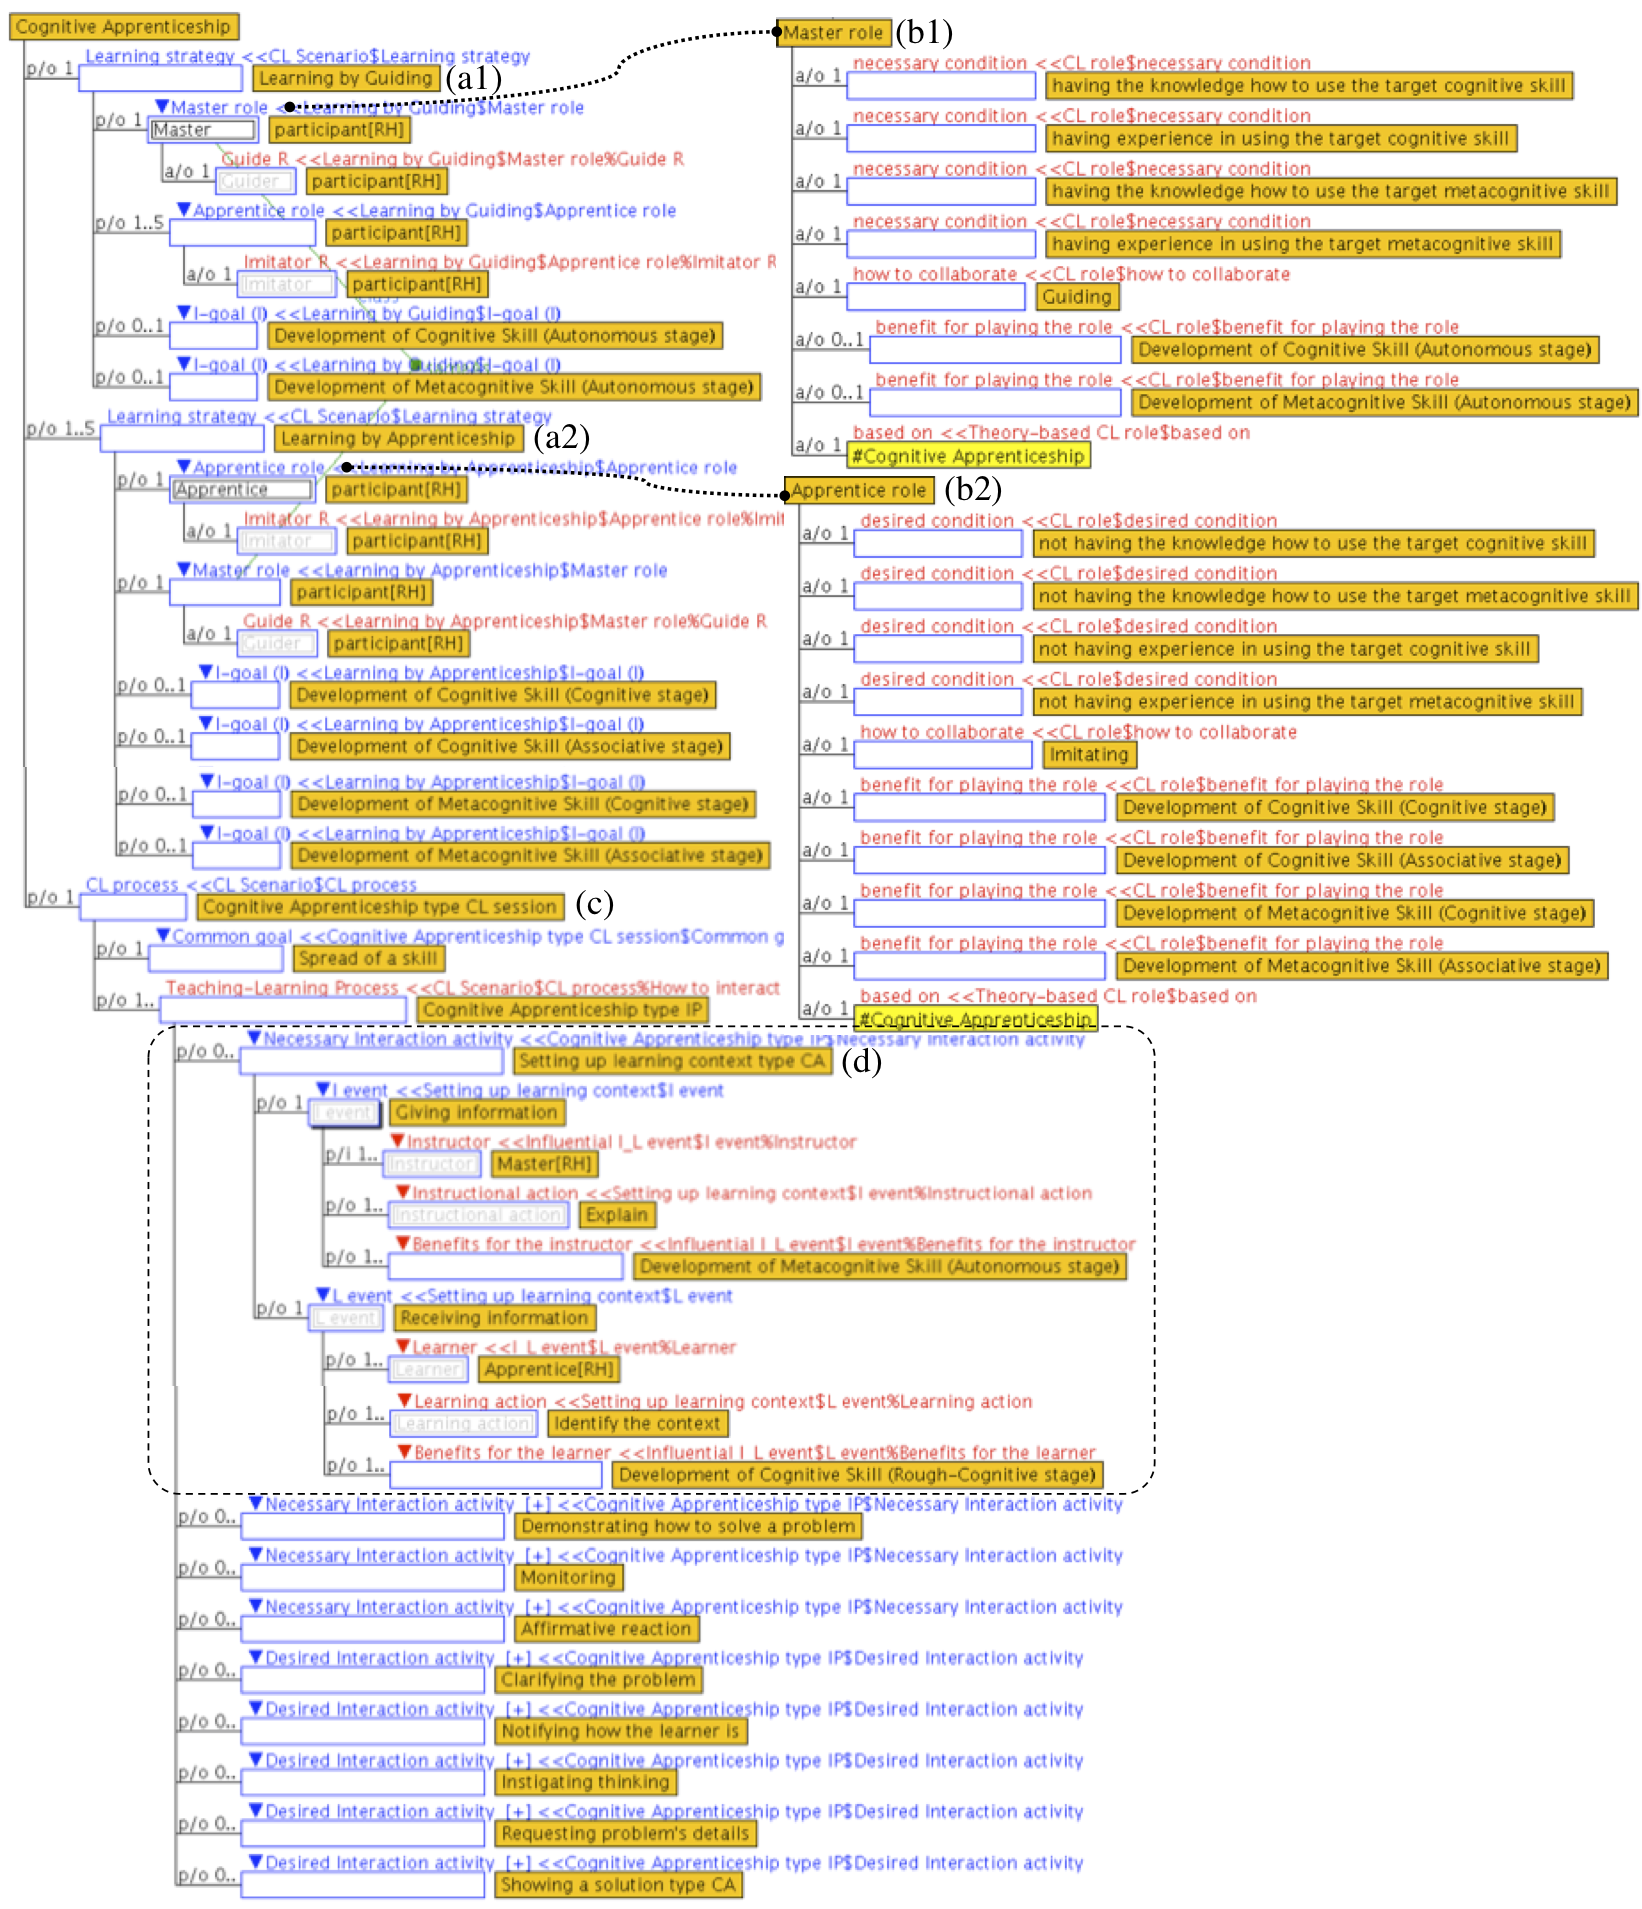
\includegraphics[width=1\textwidth]{images/chap-ontogacles1/cognitive-apprenticeship-ontological-structure.png}
 \fautor
\end{figure}

According to the cognitive apprentice theory, the more skilled participant who plays the master role must have knowledge and/or experience in using the target cognitive or metacognitive skill. Therefore, the necessary conditions to play the \emph{Master role} as shown in \autoref{fig:cognitive-apprenticeship-ontological-structure} (b1) are: \emph{having the knowledge how to use the target cognitive skill}, \emph{having experience in using the target cognitive skill}, and \emph{having experience in using the target metacognitive skill}.  When a participant adequately plays the master role, he/she acts \emph{Guiding} others participants, and as consequence of this behavior, he/she is benefited with the \emph{Development of cognitive or metacognitive skill} at the \emph{Autonomous stage}. The cognitive apprenticeship theory indicates that the participants without any knowledge or experience in how to use the target skill should play the apprentice role. Therefore, there is not necessary conditions in the ontological structure shown in \autoref{fig:cognitive-apprenticeship-ontological-structure} (b2) to represent the \emph{Apprentice role}, and the desired conditions for this role are: \emph{not having the knowledge how to use target metacognitive or cognitive skill} and \emph{not having experience in using the target metacognitive or cognitive skill}. When a participant adequately play the \emph{Apprentice role}, he/she acts \emph{Imitating} the behavior of the master and obtaining the benefits in the \emph{Development of metacognitive or cognitive skill} at the levels of \emph{Cognitive} and \emph{Associative} stages.

When the two learning strategies, \emph{Learning by Guiding} and \emph{Learning by Apprenticeship}, are simultaneously employed to structure the interactions among the participants in the CL scenario, a positive synergy is created among them producing a \emph{Spread of skills}. This arrangement is formalized by the ontological structure shown in \autoref{fig:cognitive-apprenticeship-ontological-structure} (c), where the \emph{CL process} is defined as a \emph{Cognitive Apprenticeship type CL session}, the \emph{Common goal} of this session is the \emph{Spread of skill}, and the \emph{Teaching-Learning Process} is an \emph{Interaction Pattern} defined by the sequencing mechanism of a CSCL script inspired by the Cognitive Apprenticeship theory. This sequencing mechanism defines the necessary and complementary interactions shown in \autoref{fig:cognitive-apprenticeship-cscl-script}. 

\begin{figure}[!htbp]
 \caption{Necessary and complementary interactions defined by the sequencing mechanism of a CSCL script inspired by the cognitive apprenticeship theory}
 \label{fig:cognitive-apprenticeship-cscl-script}
 \centering
 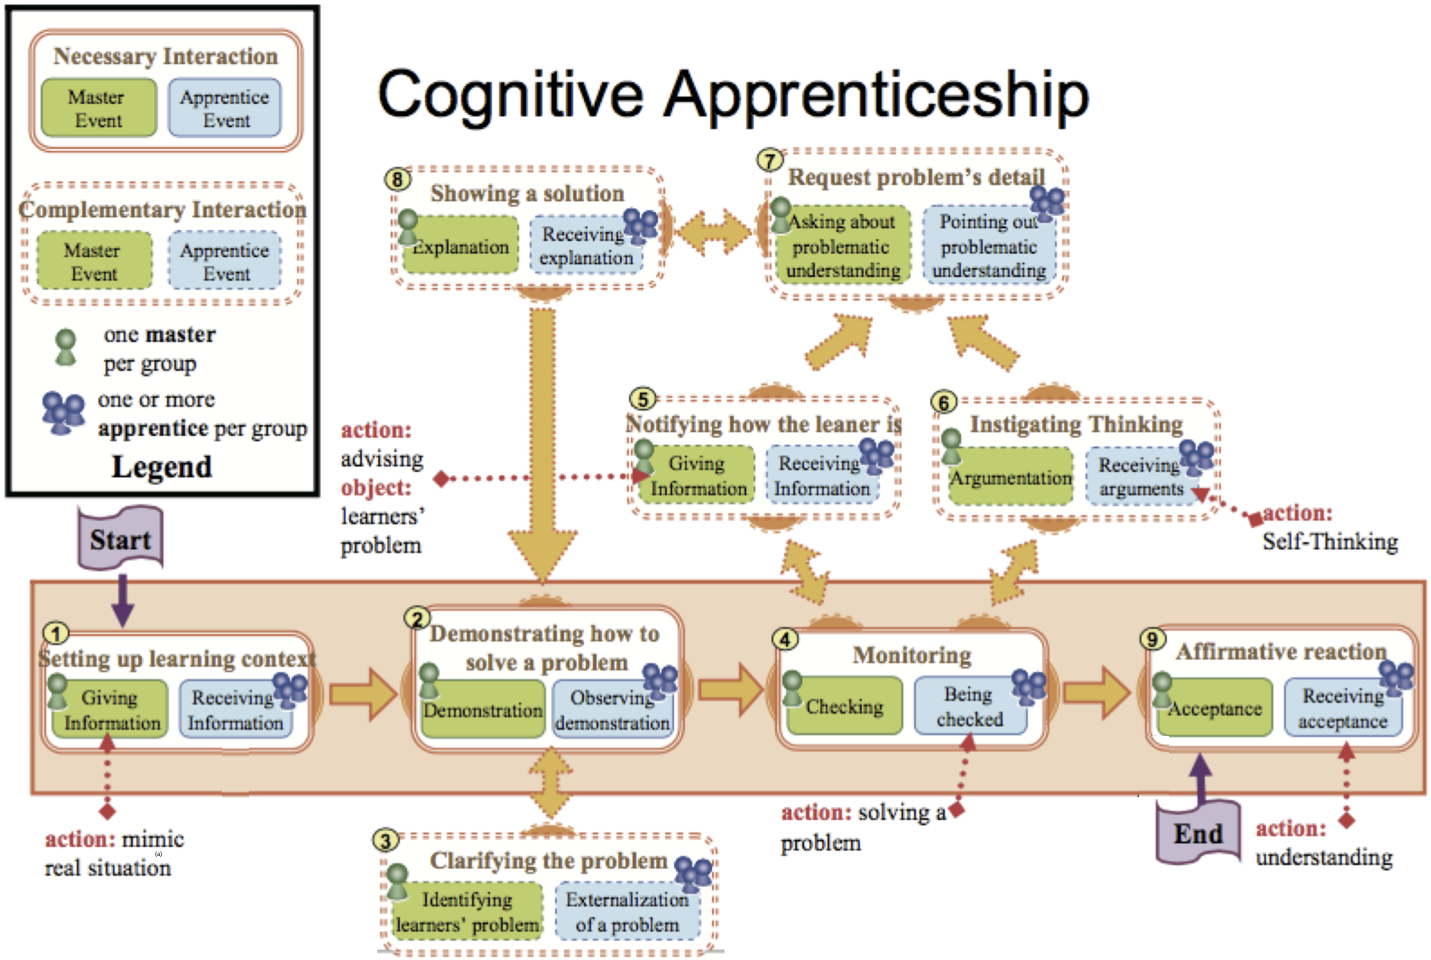
\includegraphics[width=1\textwidth]{images/chap-ontogacles1/cognitive-apprenticeship-cscl-script.png}
 \fadaptada{Isotani2009}
\end{figure}

The necessary and desired interactions defined by the sequencing mechanism shown in \autoref{fig:cognitive-apprenticeship-cscl-script} are formalized as \emph{Influential I\_L event} in the \emph{Teaching-Learning Process} of \emph{Cognitive Apprenticeship type CL session} shown in \autoref{fig:cognitive-apprenticeship-ontological-structure} (c). The ontological structure to represent the interaction \aspas{\emph{Setting up learning context type CA}} is shown in detail in \autoref{fig:cognitive-apprenticeship-ontological-structure} (d). In this interaction, the instructional event \aspas{\emph{Giving Information}} describes the action \aspas{\emph{Explain}} as an instructional action performed by the participant who plays the \emph{Master role} to \emph{develop the metacognitive skill} at the level of \emph{Autonomous stage}. The learning event \aspas{\emph{Receiving information}} describes the action \aspas{\emph{Identify the context}} as a learning action performed by the participant who plays the \emph{Apprentice role} to \emph{develop the cognitive skill} at the level of \emph{Rough-Cognitive stage}.


%%%%%%%%%%%%%%%%%%%%%%%%%%%%%%%%%%%%%%%%%%%%%%%%%%%%

\section[Ontological Structures to Represent Gamified CL Scenarios]{Ontological Structures to Represent Gamified Collaborative Learning Scenarios}
\label{sec:modeling-gamified-cl-scenarios}

The concepts, terms and relations shown in \autoref{fig:concepts-terms-and-relation-in-gamified-cl-scenarios} have been formalized in the ontology OntoGaCLeS to represent gamified CL scenarios. These elements employ an independent vocabulary from any theory and practice, and they are described as follows as:

\begin{figure}[!htbp]
 \caption{Concepts, terms and relations defined in the ontology to represent gamified CL scenarios}
 \label{fig:concepts-terms-and-relation-in-gamified-cl-scenarios}
 \centering
 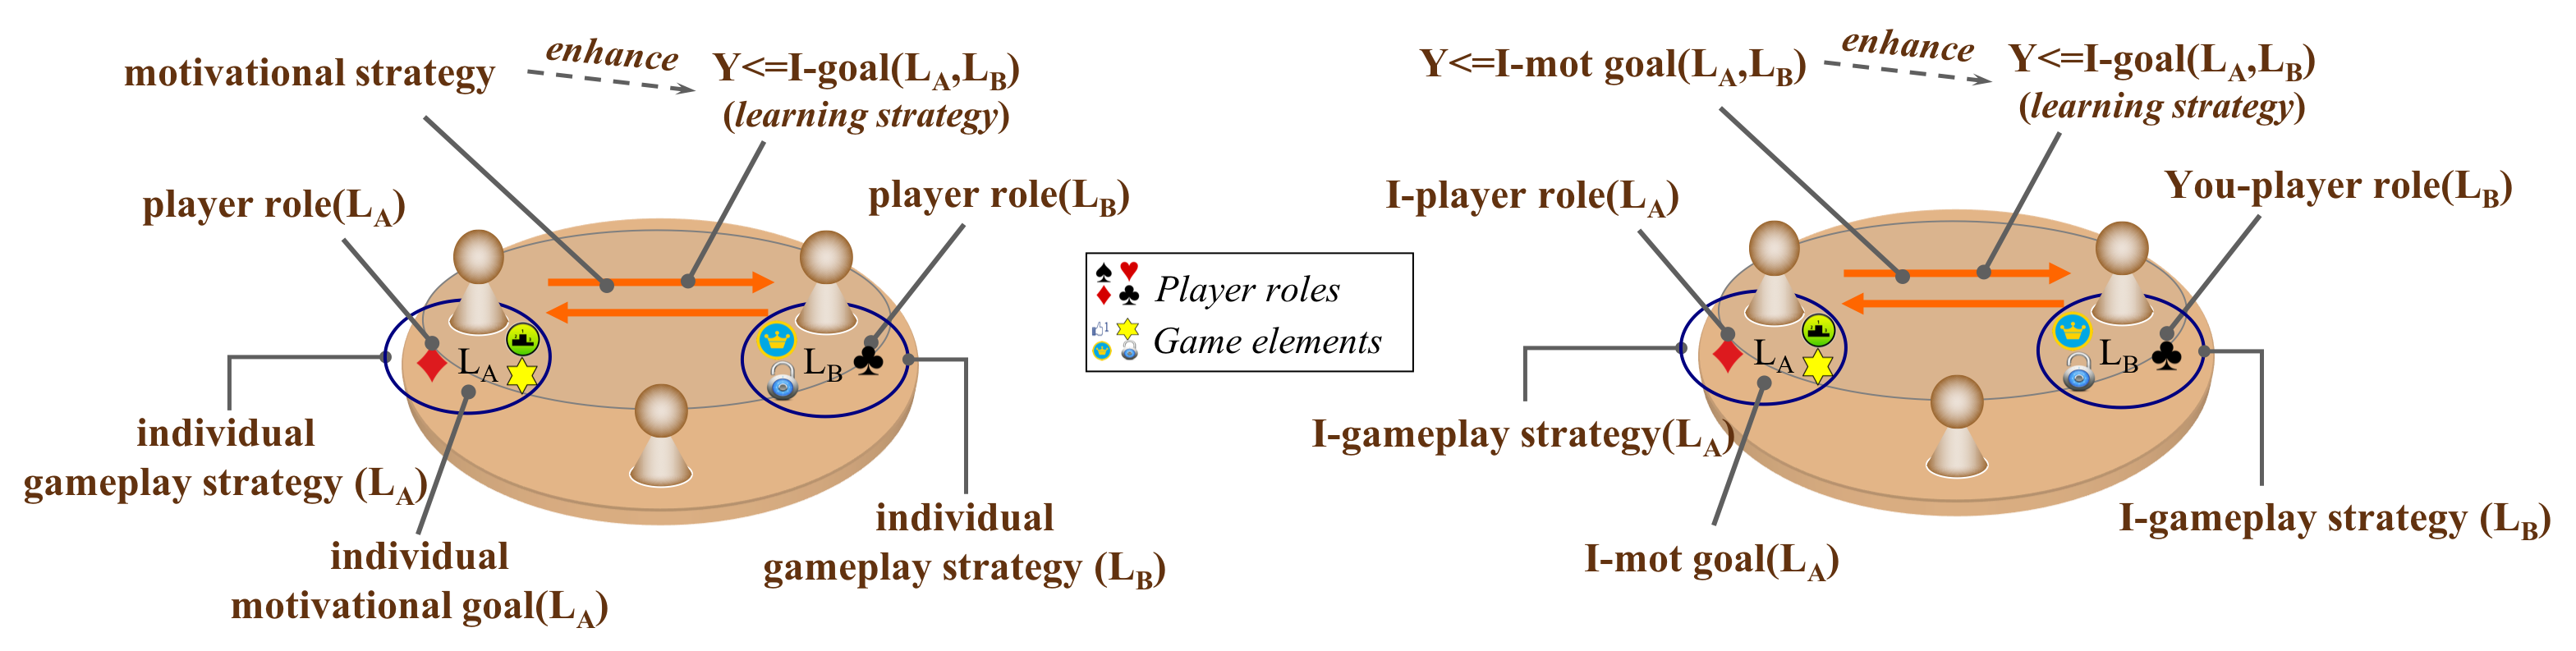
\includegraphics[width=1\textwidth]{images/chap-ontogacles1/concepts-terms-and-relation-in-gamified-cl-scenarios.png}
 \fautor
\end{figure}

\begin{description}
\item[\textbf{Y<=I-mot goal}]
is the \emph{individual motivational strategy} used to enhance the learning strategy (\emph{Y<=I-goal}) employed by the participant in focus (\emph{I}).

\item[\textbf{I-mot goal}]
is the \emph{individual motivational goal} for the participant in focus (\emph{I}), and it represents what is expected to happen in his/her motivational stage when an individual motivational strategy (\emph{Y<=I-mot goal}) is applied in the CL scenario to enhance the learning strategy (\emph{Y<=I-goal}) employed by him/her to interact with other member of group (\emph{You}).

\item[\textbf{I-player role}]
is the \emph{player role} for the participant in focus (\emph{I}).

\item[\textbf{You-player role}]
is the \emph{player role} for the participant (\emph{You}) who interacts with the participant in focus (\emph{I}).

\item[\textbf{I-gameplay}]
is the \emph{individual gameplay strategy} for the participant in focus (\emph{I}), and it describes the implementation of the individual motivational strategy (\emph{Y<=I-mot goal}) when this strategy corresponds to the gamification.
\end{description}

In the following subsections, the formalization of concepts, terms and relations briefly introduced here are detailed.

\subsection{Individual Motivational Goal (I-mot goal)}
\label{subsec:individual-motivational-goal}

The \emph{individual motivational goal} (\emph{I-mot goal}) has been formalized in the ontology OntoGaCLeS to represent the reason why is necessary to apply an individual motivational strategy in a CL scenario. Thus, for the participant in focus (\emph{I}), the individual motivational goal (\emph{I-mot goal}) represents what is expected to happen in his/her motivational stage when a motivational strategy is applied in the CL scenario to enhance the learning strategy employed by him/her to interact with others. In this sense, the individual motivational goal describes the motivational stages that must be reached by a person to be motivated to interact with other.

\autoref{fig:ontological-structure-i-mot-goal} shows the ontological structure that has been formalized in the ontology OntoGaCLeS to represent an individual motivational goal (\emph{I-mot goal}), where: the \emph{initial stage} and \emph{goal stage} are stages used to represent the expected change in the motivational stage of the person in focus (\emph{I}).

\begin{figure}[!htbp]
 \caption[Ontological structures to represent individual motivational goal (I-mot goal)]{Ontological structures to represent individual motivational goal (\emph{I-mot goal}). At the bottom, the \aspas{\emph{Satisfaction of psychological need}} (left) and the \aspas{\emph{Internalization of motivation}} (right)}
 \label{fig:ontological-structure-i-mot-goal}
 \centering
 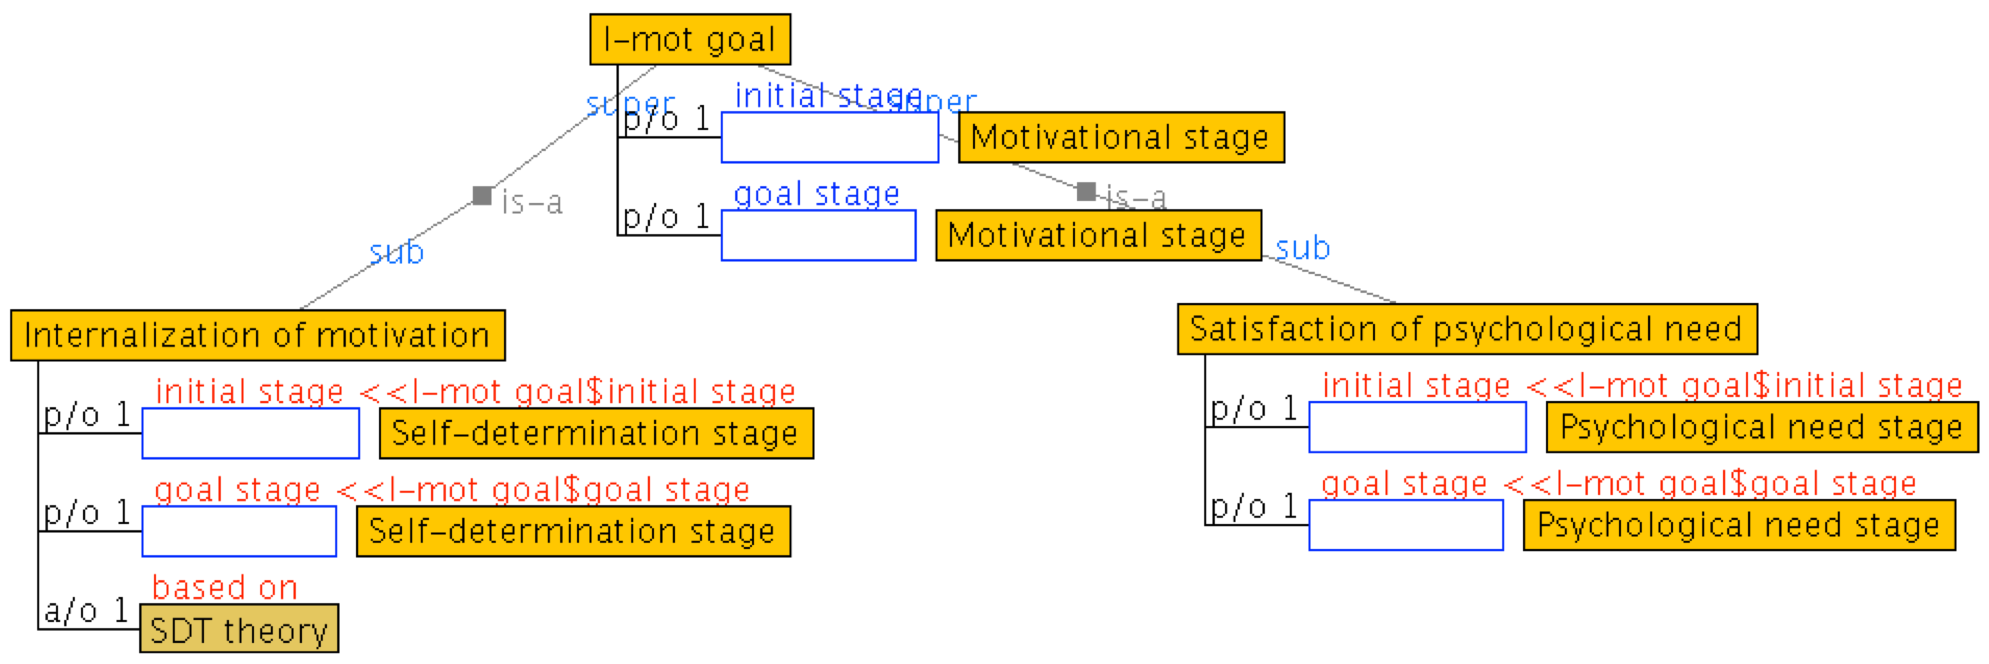
\includegraphics[width=1\textwidth]{images/chap-ontogacles1/ontological-structure-i-mot-goal.png}
 \fautor
\end{figure}

Two types of individual motivational goals have been currently formalized in the ontology OntoGaCLeS to describe the individual motivational goals (\emph{I-mot goal}) related to gamification as individual motivational strategy. The former, known as \emph{Satisfaction of psychological needs}, has been formalized based on the conceptualization of motivation as internal psychological process to satisfy human needs \cite{PritchardAshwood2008}; and the latter, known as \emph{Internalization of motivation}, has been formalized based on the form in which an individual regulates his/her own choices to behave and act \cite{DeciRyan2010}. \autoref{fig:ontological-structure-i-mot-goal} shows the representation for these two types of individual motivational goals. The initial and goal stages related to the \emph{Internalization of motivation} are defined by the self-determination stage, whereas the initial and goal stages for the \emph{Satisfaction of psychological need} are defined by the \emph{psychological need stages}. In the articles  \cite{ChallcoMoreiraBittencourtMizoguchiIsotani2015, ChallcoMoreiraMizoguchiIsotani2014, ChallcoMoreiraMizoguchiIsotani2014a}, the author of this thesis used the concept of \aspas{\emph{Phychological need}} to refer the concept of \aspas{\emph{Psychological need stage},} and the concept of \aspas{\emph{Without need}} to refer the stages described as \aspas{\emph{\$1 need satisfied}} where \$1 is substitute by psychological needs (e.g. \emph{Mastery need satisfied}).

As it was mentioned before, in the \autoref{chapter:general-background}, motivation is an internal psychological process associated with three general components of arousal, direction and intensity in which the arousal component is caused by needs (also called \emph{wants} or \emph{desires}). These needs cause that a person behaves and acts to satisfy needs \cite{MitchellDaniels2003}. Consequently, motivation is a constructor that describes why a person chooses to allocate time and energy for different behaviors and actions to maximize the satisfaction of his/her own needs \cite{PritchardAshwood2008}. It means that, in a CL scenario, the motivation problem caused by the scripted collaboration occurs when the participant believes that this scenario will not lead him/her to satisfy his/her individual needs. Therefore, the motivational strategy is applied in the CL scenario to change this perception. Based on this assumption, the individual motivational goals (\emph{I-mot goal}) for the person in focus (\emph{I}) has been formalized in the ontology OntoGaCLeS as the satisfaction of needs. More specifically, in gamified CL scenarios, the individual motivational goal is described as \emph{Satisfaction of psychological needs} because game elements do not satisfy all human needs, they only satisfy part of these needs that are referred by the author of this thesis as \emph{psychological needs}. The psychological needs are the human needs that are classified in the groups of relatedness and growth needs according to the ERG (Existence, Relatedness and Growth) theory \cite{Alderfer1972}.

\begin{figure}[!htbp]
 \caption[Ontological structures to represent satisfaction of psychological need]{Ontological structures to represent \aspas{\emph{Satisfaction of psychological need}.} At the top right, the ontological structure to represent \aspas{\emph{Satisfaction of autonomy}.}}
 \label{fig:ontological-structure-satisfaction-psychological-need}
 \centering
 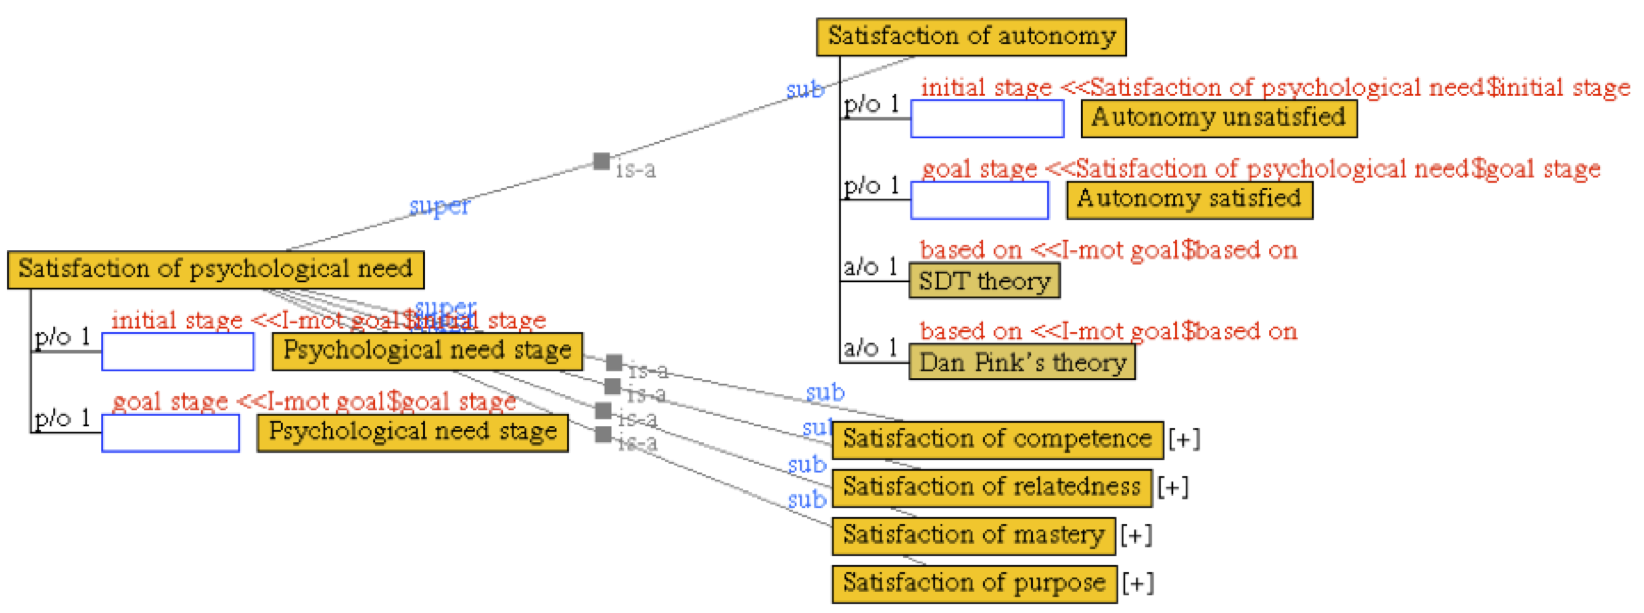
\includegraphics[width=1\textwidth]{images/chap-ontogacles1/ontological-structure-satisfaction-psychological-need.png}
 \fautor
\end{figure}

\autoref{fig:ontological-structure-satisfaction-psychological-need} shows the ontological structures formalized to represent the \emph{Satisfaction of psychological need}. These ontological structures represent the satisfaction of innate psychological needs, and they comprise what is intended to evoke in minds of users by the majority of experts when non-game contexts are gamified \cite{MoraRieraGonzalezArnedo-Moreno2015, SeabornFels2015}. According to the SDT theory \cite{RyanDeci2000,DeciRyan2010}, the well-being of an individual is reached when the psychological needs of autonomy, competence and relatedness are satisfied \cite{DeciRyan1985, DeciRyan2010}, and according to the Dan Pink's theory \cite{Pink2011}, a person is motivate and engage in a cognitive, decision-making, creative or higher-order thinking task when it is given with autonomy, mastery and purpose. At the top right of \autoref{fig:ontological-structure-satisfaction-psychological-need}, the ontological structure to represent the \emph{Satisfaction of autonomy} is detailed in which, based on a unipolar scale from unsatisfied need to satisfied need, the roles for the initial and goal stages are played by the \emph{Autonomy unsatisfied} and the \emph{Autonomy satisfied}, respectively. Employing the same unipolar scale, and the need-theories of motivation, SDT theory \cite{DeciRyan2010} and Dan Pink motivation theory \cite{Pink2011}, a set of individual motivational goals as satisfactions of psychological needs have been formalized in the ontology OntoGaCLeS, and they are detailed in \autoref{sec:ontogacles:i-mot-goal}.

\begin{figure}[!htbp]
 \caption[Ontological structures to represent internalization of motivation]{Ontological structures to represent \aspas{\emph{Internalization of motivation}.} At the top right, the ontological structure to represent the \aspas{\emph{Internalization from amotivation to intrinsic motion}.}}
 \label{fig:ontological-structure-internalization-motivation}
 \centering
 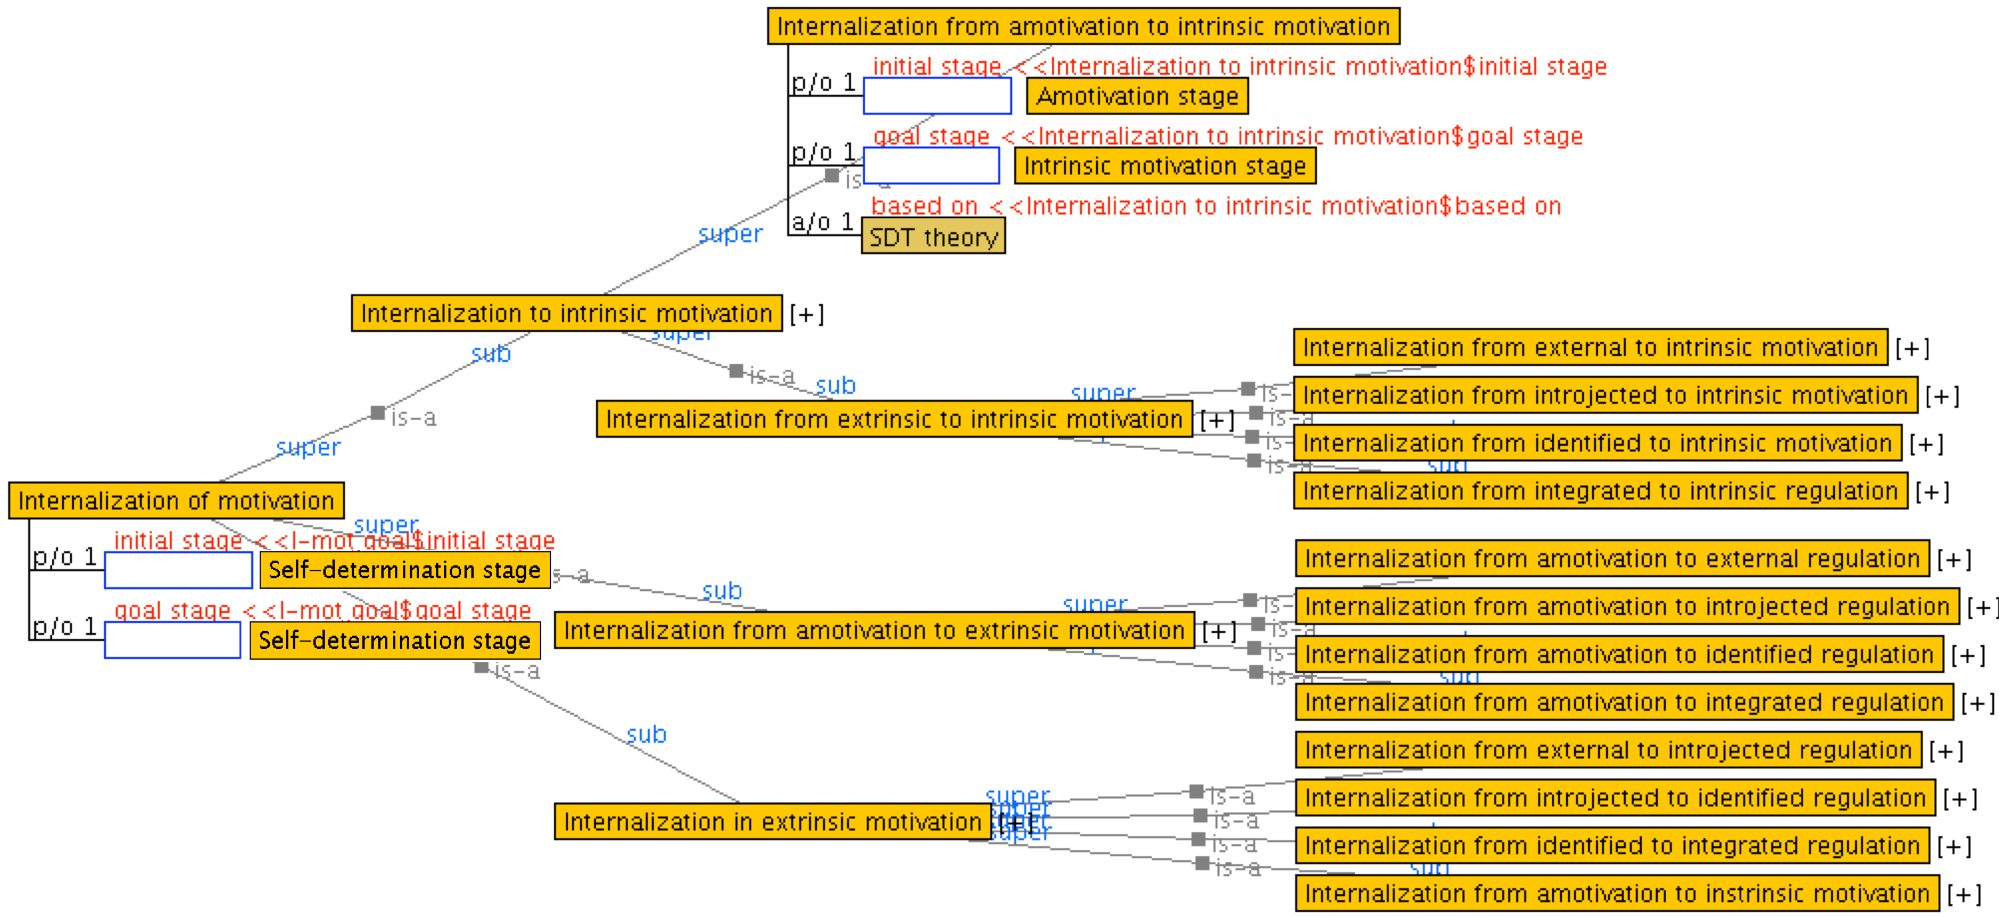
\includegraphics[width=1\textwidth]{images/chap-ontogacles1/ontological-structure-internalization-motivation.png}
 \fautor
\end{figure}

The \emph{internalization of motivation} is the process by which \aspas{\emph{values, attitudes or regulatory structures, such that the external regulation of a behavior is transformed into an internal regulation, so no longer requires the presence of an external contingency}} \cite{GagneDeci2005}. In this sense, the internalization of motivation in relation to the satisfaction of needs refers to changes in the motivation from a non-free choice to a free choice of needs that are satisfied by oneself. According to the SDT theory \cite{DeciRyan1985, RyanDeci2000}, this change happens from the extrinsic motivation to intrinsic motivation when motivation is changed from a non-self-determined form (\emph{non-freely choice}) to a self-determined form (\emph{freely choice by oneself}). Here, the extrinsic motivators employed by the game elements must be configured as an attempt to transform the current motivation stages of participants from amotivation and extrinsic motivation into intrinsic motivation. Based on these definitions, the ontological structures shown in \autoref{fig:ontological-structure-internalization-motivation} have been formalized in the ontology OntoGaCLeS to represent the \emph{Internalization of motivation}. These ontological structures have been formalized employing the continuum ranging of stages from \emph{amotivation} (not internalized behave) into \emph{external motivation} (not at all internalized behave) to \emph{introjected motivation} (partially internalized behave) to \emph{identified motivation} (fully internalized behave) to \emph{intrinsic motivation} (automatically internalized behave). At the top right of \autoref{fig:ontological-structure-internalization-motivation} is detailed the formalization for the change from \emph{Amotivation stage} (\emph{initial stage}) to \emph{Intrinsic motivation stage} (\emph{goal stage}) defined as \aspas{\emph{Internalization from amotivation to intrinsic motivation}.} The detailing of all ontological structures to represent the internalization of motivation is presented in \autoref{sec:ontogacles:i-mot-goal}.

\subsection{Player Role}
\label{subsec:player-role}

The identification of homogeneous people groups that differ from other groups in a significant way is essential to define the personalization in any system. In game design, this segmentation is established by player types models in which typologies are used to categorize the users in different groups according to their geographic location \cite{BenJuddChrisAvelloneHideoKojimaKeijiInafune2016, ChakrabortyNorcioVeerAndreMillerRegelsberger2015}, their demographic situation \cite{GreenbergSherryLachlanLucasHolmstrom2010, Shaw2012}, their psychographic characteristics \cite{Tseng2011, Yee2006}, and their behavioral characteristics \cite{Bartle2004, Lazzaro2009}. These player type models aim to help the game designers to identify the necessary features that make a game fun, enjoyable and desirable for a particular audience.

The player type models cannot be directly extrapolated to others context for which they are not intended. Thus, the concept of \emph{Player role} has been formalized by the author of this thesis in the ontology OntoGaCLeS to define typologies of player types in the context of CL scenarios. Player roles describe the functionality, responsibilities and requirements whereby a group of participants becomes players in a gamified CL scenario. This segmentation is based on individual characteristics of participants that establish a segmentation of participants using necessary and desired conditions. In this sense, the \emph{Player role} has been formalized by the ontological structure shown in \autoref{fig:ontological-structure-player-role}. This structure defines the conditions that must be satisfied by a participant in the CL scenario to play the player role as: \emph{necessary condition} and \emph{desired condition}. Thus, a participant of CL scenario cannot play a player role when he/she does not fulfill the necessary conditions, and when the participant fulfills the necessary and desired conditions has more probability to obtain the expected \emph{benefits for playing the role}.

The necessary and desire conditions in the ontological structure to represent \emph{Player role} are defined by: motivation states, psychological need states, and individual personality trait states. A tree overview for these states are detailed in \autoref{sec:ontogacles:tree-overview-states}, where:

\begin{itemize}
\item
The \emph{motivation state} is an internal state that describes the temporal attitudinal state of a person in relation to his/her desire to be a participant in the CL session. These stages can be \emph{Not motivated} and \emph{Motivated}. The state of motivated is also divided in two types: \aspas{\emph{Intrinsic motivated}} and \aspas{\emph{Extrinsic motivated}} \cite{DeciRyan2010}. It is important to notice here that the concept of motivation state is not the same as the concept of motivation stage. Although both concepts represent changes in relation to the motivation of participants, the motivation state represents a specific point in the whole process of being motivated, whereas the motivation stage represents an interval in the motivation process.

\item
The \emph{psychological need state} represents the current psychological need of a person in which the states for each one of the psychological needs are formalized through the representation of pair states: \aspas{\emph{Having need of \$1}} and \aspas{\emph{Not having need of \$1}} in which \aspas{\emph{\$1}} is replaced by the name of the need that is being described as prerequisite. For instance, to represent the states related to the psychological need of competence, the states of \aspas{\emph{Having need of competence}} and \aspas{\emph{Not having need of competence}} have been formalized as psychological need state in the ontology OntoGaCLeS.

\item
The \emph{individual personality trait state} describes states related to individual personality traits, such as introversion, extraversion, openness to experience, and conscientiousness. The individual personality trait states describe the characteristic that make a person unique by indicating his/her habitual patterns of thought, emotion and behavior for different situations \cite{MatthewsDearyWhiteman2003}. These states express whether a participant either has or does not have the individual personality trait. In the ontology OntoGaCLeS, there are represented individual personality traits states related to: the big five personality traits \cite{CostaMacCrae1992}, the MBTI personality traits \cite{Briggs1976}, the game-playing style preferences described in the Bartle's player type model \cite{Bartle2004}, and the game-playing liking preferences described in the Yee's motivation components \cite{Yee2006}.
\end{itemize}

\begin{figure}[!htbp]
 \caption[Ontological structure to represent player role]{Ontological structure to represent \aspas{\emph{Player role}} (At the top). At the bottom, the ontological structure to represent the player role \aspas{\emph{Dreamer role}.}}
 \label{fig:ontological-structure-player-role}
 \centering
 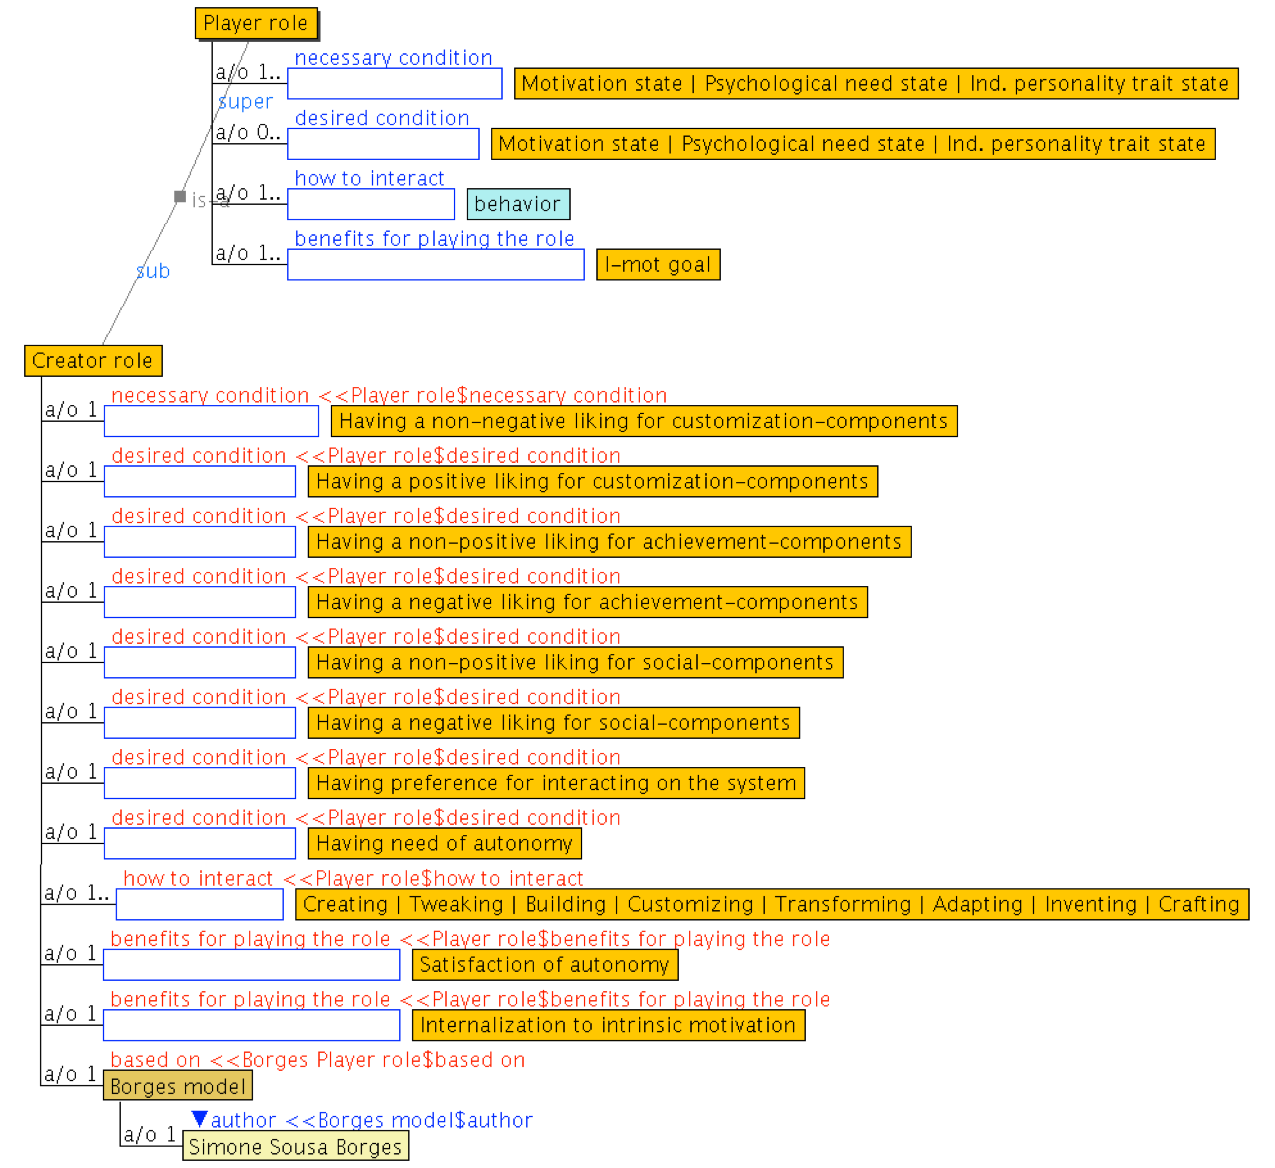
\includegraphics[width=1\textwidth]{images/chap-ontogacles1/ontological-structure-player-role.png}
 \fautor
\end{figure}

Beside to describe the necessary and desired conditions that should be satisfied by an individual, the ontological structure to represent \emph{Player role} shown in \autoref{fig:ontological-structure-player-role} describe the information about: how the participant with the player role is expected to interact with the game elements (\emph{how to interact}), and the expected benefits for playing the player role (\emph{benefits for playing the role}). Thus, concepts described as \emph{behavior} are used to represent the possible manners in which a participant should interact to other, and concepts described as individual motivational goals (\emph{I-mot goal}) are used to represent the expected \emph{benefits for playing the role}.

At the bottom of \autoref{fig:ontological-structure-player-role}, the \emph{Creator role} is shown as example of the formalization of a player role using the ontological structure proposed in this section. According to this structure, participants who have a greater liking for customization-components rather than for other game components are classified as creators. This segmentation is represented by the necessary condition of \aspas{\emph{having a non-negative liking for customization-components},} and the desired conditions of \aspas{\emph{having a positive liking for customization-components},} \aspas{\emph{having a non-positive liking for achievement-component},} \aspas{\emph{having a negative liking for achievement-component},} \aspas{\emph{having a non-positive liking for social-component},} and \aspas{\emph{having a negative liking for social-component}.} The desired conditions related to the behavioral characteristics of participants to act as a player role are: \aspas{\emph{having preference for interacting on the system}} and \aspas{\emph{having need of autonomy}.} The expected behaviors to obtain benefits for playing the creator role are: \aspas{\emph{Creating},} \aspas{\emph{Tweaking},} \aspas{\emph{Building},} \aspas{\emph{Customizing},} \aspas{\emph{Transforming},} \aspas{\emph{Adapting},} \aspas{\emph{Inventing}} or \aspas{\emph{Crafting}.} As consequence to behave as creator, the participants attain the \emph{Satisfaction of autonomy} and the \emph{Internalization to intrinsic motivation} (\emph{I-mot goal}).

In the ontology OntoGaCLeS, based on the information extracted from five different player type models, twenty-six players roles have been formalized and represented using the ontological structure proposed in this section. These player roles, their conditions, expected behaviors and benefits for the person who plays the role are detailed in \autoref{sec:ontogacles:player-role}.

\subsection{Individual Motivational Strategy (Y<=I-mot goal)}

In the context of CL scenarios, an \emph{individual motivational strategy} is defined by the author of this thesis as a set of guidelines defined to motivate a participant to interact with other group members using learning strategies. These guidelines are independent of any technology, so that the individual motivational strategy basically describes what motivates a participant to act and behave in certain way. For example, consider the following guidelines extracted from the Model-driven Persuasive Game in which:

\begin{citacao}
\aspas{... cooperation is only a significant motivator of behaviour change for achievers and socializers... This is in line with the gaming style of socializers, who enjoy helping others. Achievers would also prefer to cooperate because they are inherently more altruistic ... achievers do often co-operate with one another, usually to perform some difficult collective goal, and from these shared experiences can grow deep, enduring friendships which may surpass in intensity those commonly found among individuals other groups.} \citeonline{Orji2014}.
\end{citacao}

When these two guidelines are applied in a CL scenario by providing a situation in which the participants must cooperate to achieve a group goal (e.g. obtain a especial reward based on the collective performance of group members), these guidelines becomes a individual motivational strategy that could be applied to motivate participant who fall in the category of socializer or achiever because they are motivated by the desired to accomplish the group goal and the desired to help others, respectively.

The ontological structure shown in \autoref{fig:ontological-structure-individual-motivational-strategy} has been proposed by the author of this PhD thesis dissertation to represent the formalization of individual motivational strategies whose guidelines are extracted from gamification models or game design models. According to this structure, an \emph{individual motivational strategy} (\emph{Y<=I-mot goal}) is described by:

\begin{description}
\item[\textbf{I-player role}]
to indicate the player role for the participant in focus (\emph{I}) who becomes a \emph{player role holder} when he/she is motivated by the motivational strategy. This player role also indicates the \emph{behavioral roles} whereby the participant in focus (\emph{I}) is motivated to interact with other participant (\emph{You}) employing the learning strategy (\emph{Y<=I-goal}).

\item[\textbf{You-player role}]
to indicate the player role for the participant (\emph{You}) who interacts with the participant in focus (\emph{I}). The \emph{behavioral roles} whereby the \emph{player role holder} of this role supports the interaction of participant in focus (\emph{I}) are also indicated in this structure.

\item[\textbf{I-mot goal (I)}]
to indicate the individual motivational goals (\emph{I-mot goal (I)}) whereby the participant in focus (\emph{I}) is motivated to interact with other participant (\emph{You}) employing a learning strategy (\emph{Y<=I-goal}). In this sense, these individual motivational goals represent the reasons why the guidelines contained in the motivational strategy are applied in the CL scenario to enhance the learning strategy (\emph{Y<=I-goal}) employed by the participant in focus (\emph{I}) to interact with other participant (\emph{You}).
\end{description}

\begin{figure}[!htbp]
 \caption[Ontological structure to represent individual motivational strategy]{Ontological structure to represent \aspas{\emph{Individual motivational strategy}} (at the left). At the right, the motivational strategies \aspas{\emph{Gamifying for Consumer and Dodecad Achiever}} (right-top) and \aspas{\emph{Gamifying by COOP}} (right-bottom).}
 \label{fig:ontological-structure-individual-motivational-strategy}
 \centering
 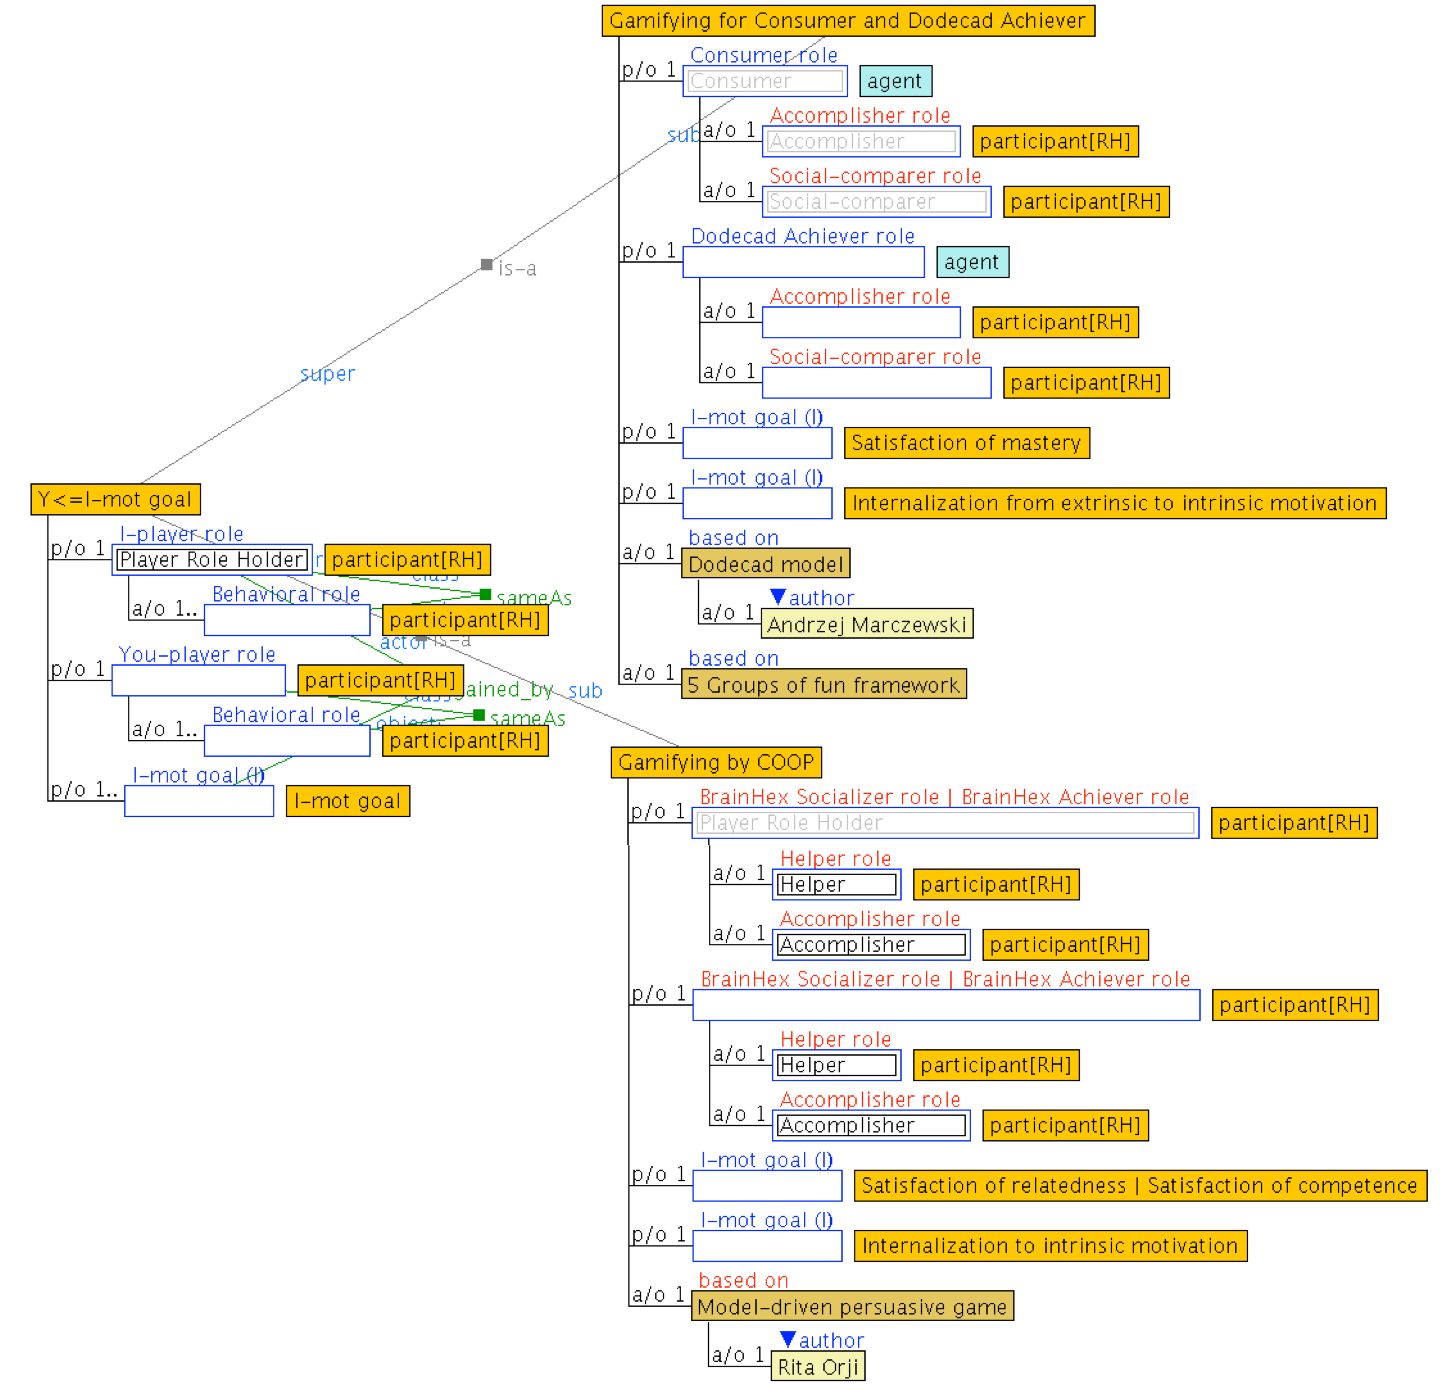
\includegraphics[width=1\textwidth]{images/chap-ontogacles1/ontological-structure-individual-motivational-strategy.png}
 \fautor
\end{figure}

To exemplify the formalization of the individual motivational strategies using the ontological structure proposed in this section, \autoref{fig:ontological-structure-individual-motivational-strategy} also shows two examples in which the attribute \aspas{\emph{based on}} indicates the gamification models in which these motivational strategies are based. The individual motivational strategy shown at the top-right of \autoref{fig:ontological-structure-individual-motivational-strategy} is known as \aspas{\emph{Gamifying for Consumer and Dodecad Achiever},} and it has been formalized based on guidelines of the Dodecad model \cite{Marczewski2015a} and 5 Groups of fun framework \cite{Marczewski2015b}. According to these guidelines, the consumers and achievers are motivated by the need to obtain a reward that demonstrates for other participants their accomplishments. Hence, the \emph{Accomplisher} and \emph{Social-comparer} are \emph{behavioral roles} whereby a participant in focus (\emph{I}) playing the \emph{Consumer role} is motivated to interact with the participant (\emph{You}) who plays the \emph{Achieve role}. Playing this role, the \emph{Satisfaction of mastery} and the \emph{Internalization from extrinsic to intrinsic motivation} are individual motivational goals whereby the participant in focus (\emph{I}) as consumer is motivated to interact with other participant (\emph{You}) who acts as achiever. Behaving as accomplisher and social-comparer, the participant in focus (\emph{I}) has two individual motivational goals that are: to demonstrate his/her mastery represented as \aspas{\emph{Satisfaction of mastery};} and to internalize his/her current extrinsic motivation stage into intrinsic motivation stage represented as \aspas{\emph{Internalization from extrinsic to intrinsic motivation}.}

At the bottom-right of \autoref{fig:ontological-structure-individual-motivational-strategy}, it is shown the ontological structure formalized to represent the application of the guidelines described in the Model-driven persuasive game for the cooperation strategy \cite{OrjiVassilevaMandryk2014}. These guidelines indicate cooperation as significant motivator for a participant who plays the socializer or achiever role because a participant who plays these roles enjoys to help others and cooperate with others in order to accomplish a difficult collective goal. Based on this, the motivational strategy of \aspas{\emph{Gamifying by COOP}} defines the \emph{BrainHex Socializer role} and \emph{Brainhex Achiever role} as player roles that would be played by the participant in focus (\emph{I}) and the participant (\emph{You}) who gives support to the participant in focus. Playing these roles, the participants (\emph{I} and \emph{You}) act as \emph{Helper} and \emph{Accomplisher}. When the participant in focus (\emph{I}) has the desire to accomplish the difficult collective goal, his/her individual motivational goal is the \emph{Satisfaction of competence}, and when the participant in focus (\emph{I}) has the desire to help others, his individual motivational goal is the \emph{Satisfaction of relatedness}. The ontological structure also describes that as consequence of the application of the motivational strategy, it is expected changes in the motivational state for the participant in focus (\emph{I}) from the amotivation or extrinsic motivated state to the intrinsic motivated state (\emph{Internalization to intrinsic motivation}).

The individual motivational strategies based on gamification models currently defined in the ontology OntoGaCLeS, their player roles, their behavioral roles, and their individual motivational goals are detailed in \autoref{sec:ontogacles:individual-motivational-strategy}.

\subsection{Individual Gameplay Strategy (I-gameplay strategy)}
\label{sec:individual-gameplay-strategy}

The guidelines extracted from the literature of gamification, game design and serious games are implemented through the design of way in which the users will experience their interactions with the game-like system \cite{FabricatoreLopez2014, NackeDrachenGobel2010, Schell2008}. Such design in gamification is frequently called as gameful design \cite{DeterdingDixonKhaledNacke2011, DichevDichevaAngelovaAgre2014}, and it has been formalized by the author of this thesis under the concept of \emph{individual gameplay strategy} (\emph{I-gameplay strategy}). In this sense, the gameplay of a gamified CL scenario is defined by the way in which the interactions between the participants and the game elements could occur. When a participant interacts with the game elements, the rules defined in the gamified CL scenario process his/her inputs causing changes in the game elements, and these modifications are communicated to the participant. These rules and changes are related to individual motivational goals that must be achieved by the participants, so that each participant has his/her own strategy to interact with the gamified CL scenario to achieve these goals. This strategy of interaction is the individual gameplay strategy, and it has been formalized by the ontological structure shown in \autoref{fig:ontological-structure-individual-gameplay-strategy}.

\begin{figure}[!htbp]
 \caption[Ontological structure to represent individual gameplay strategy]{Ontological structure to represent \aspas{\emph{Individual gameplay strategy}} (at the top). At the bottom, the \aspas{\emph{Coop. CMPT gameplay strategy}} (bottom-left), and the \aspas{\emph{Achievement fun gameplay strategy}} (bottom-right)}
 \label{fig:ontological-structure-individual-gameplay-strategy}
 \centering
 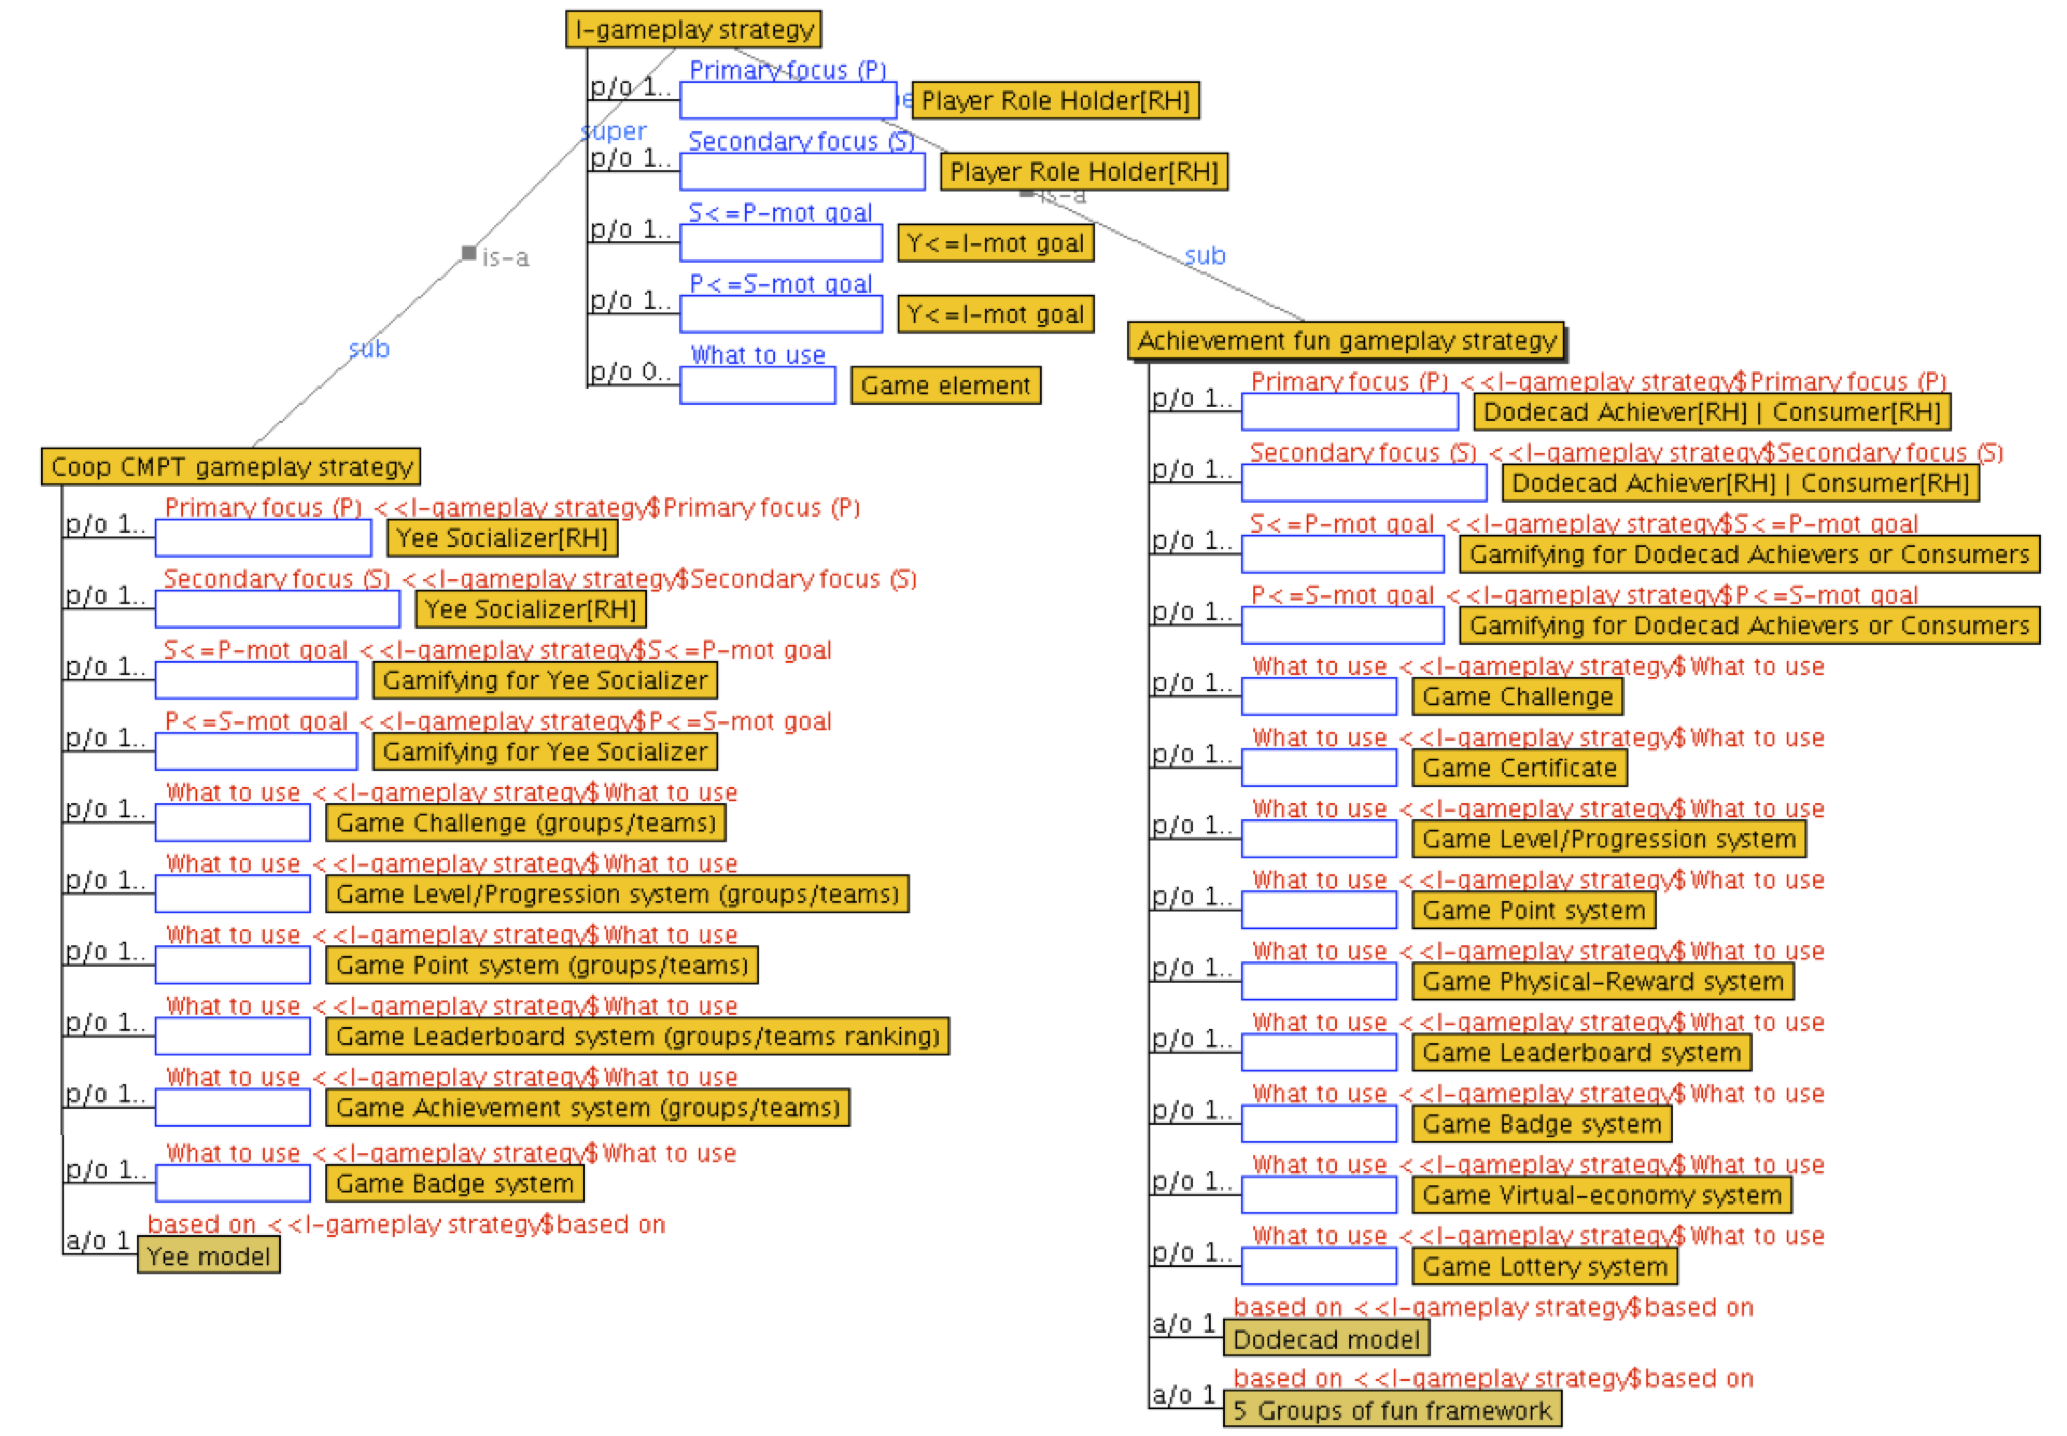
\includegraphics[width=1\textwidth]{images/chap-ontogacles1/ontological-structure-individual-gameplay-strategy.png} 
 \fautor
\end{figure}

The individual gameplay strategy depends of the player roles assigned for the participants of CL scenario, the motivational strategies employed to gamify the CL scenario, and the game elements introduced in the CL scenario. Thus, the ontological structure to represent an individual gameplay strategy is defined as a rational arrangement of these elements, where:

\begin{description}
\item [\textbf{Primary focus (P)}]
indicates the \emph{Player role holders} who are in the primary focus (P) of individual gameplay strategy. These player role holders are the participants who use the individual gameplay strategy (\emph{I-gameplay strategy}) to interact with the game elements indicated in the attribute \aspas{\emph{What to use}.}

\item [\textbf{Secondary focus (S)}]
indicates the \emph{Player role holders} who are in the secondary focus (S) of individual gameplay strategy. These player role holders are the participants who provide support for the player role holders in the primary focus (P) through the game elements indicated in the attribute \aspas{\emph{What to use}.} It means that the individual gameplay strategy (\emph{I-gameplay strategy}) is not necessary used by the participants in secondary focus (S) to interact with the game elements, but their interactions in the gamified CL scenario produce changes in the state of game elements indicated in the attribute \aspas{\emph{What to use}.}

\item[\textbf{S<=I-mot goal}]
indicates the motivational strategies employed in the gamified CL scenario to motivate the player role holders who are in the primary focus (P).

\item[\textbf{P<=S-mot goal}]
indicates the motivational strategies employed in the gamified CL scenario to motivate and engage the player role holders who are in the secondary focus (S).

\item[\textbf{What to use}]
indicates the game elements that are needed to carry out the individual gameplay strategy. Thus, the game elements defined in this attribute are the ones that are used to process the interactions of participants who are in the primary focus (P).
\end{description}

Currently, in the literature of gamification and game design, there is no one set of gameplay strategies established that could be directly formalized as individual gameplay strategies employing the ontological structure (\emph{I-gameplay strategy}) proposed here. Therefore, the author of this thesis has inferred some individual gameplay strategies employing the guidelines of gamification and game design models. \autoref{fig:ontological-structure-individual-gameplay-strategy} shows two examples of this formalization in which the guidelines described in the Yee's model \cite{Yee2006} have been used to formalize the cooperative competition gameplay strategy (\emph{Coop. CMPT gameplay strategy}) shown at the bottom-left of figure. According to this structure, a cooperative competition gameplay strategy is beneficial for participants who are holders of Yee's Socializer role, Primary focus (P), when the motivational strategy \aspas{\emph{Gamifying for Yee Socializer}} is applied in a CL scenario to motivate these group of participants to interact with other participants who are also holders of Yee's Socializer role, Secondary focus (S). In the attribute \aspas{\emph{What to use},} this structure also indicates that game challenges for groups/teams, game level/progression systems for groups/teams, game point system for groups/teams, game leaderboard system with groups/teams rankings, game achievement system for groups/teams, and game badge systems are necessary to implement the cooperative competition gameplay strategy.

\subsection{Gamified CL Scenario}
\label{subsec:gamified-cl-scenario}

A gamified CL scenario is a CL scenario in which the concepts previously presented in this section have been properly applied to gamify it. In this sense, to formally represent a gamified CL scenario in the ontology OntoGaCLeS, the ontological structures proposed in the CL ontology to represent a CL scenario (\autoref{fig:ontological-structure-cl-scenario}) has been extended by adding the representation of motivational strategies (\emph{Y<=I-mot goal}) and gameplay strategies (\emph{I-gameplay strategy}) at the same level that the learning strategies (\emph{Y<=I-goal}). The proper connection of these elements represents a \aspas{\emph{Gamified CL Scenario}} by the ontological structures shown in \autoref{fig:ontological-structure-gamified-cl-scenario}.

\begin{figure}[!htbp]
 \caption[Ontological structures to represent a gamified CL scenario]{Ontological structures to represent a \aspas{\emph{Gamified CL Scenario}}}
 \label{fig:ontological-structure-gamified-cl-scenario}
 \centering
 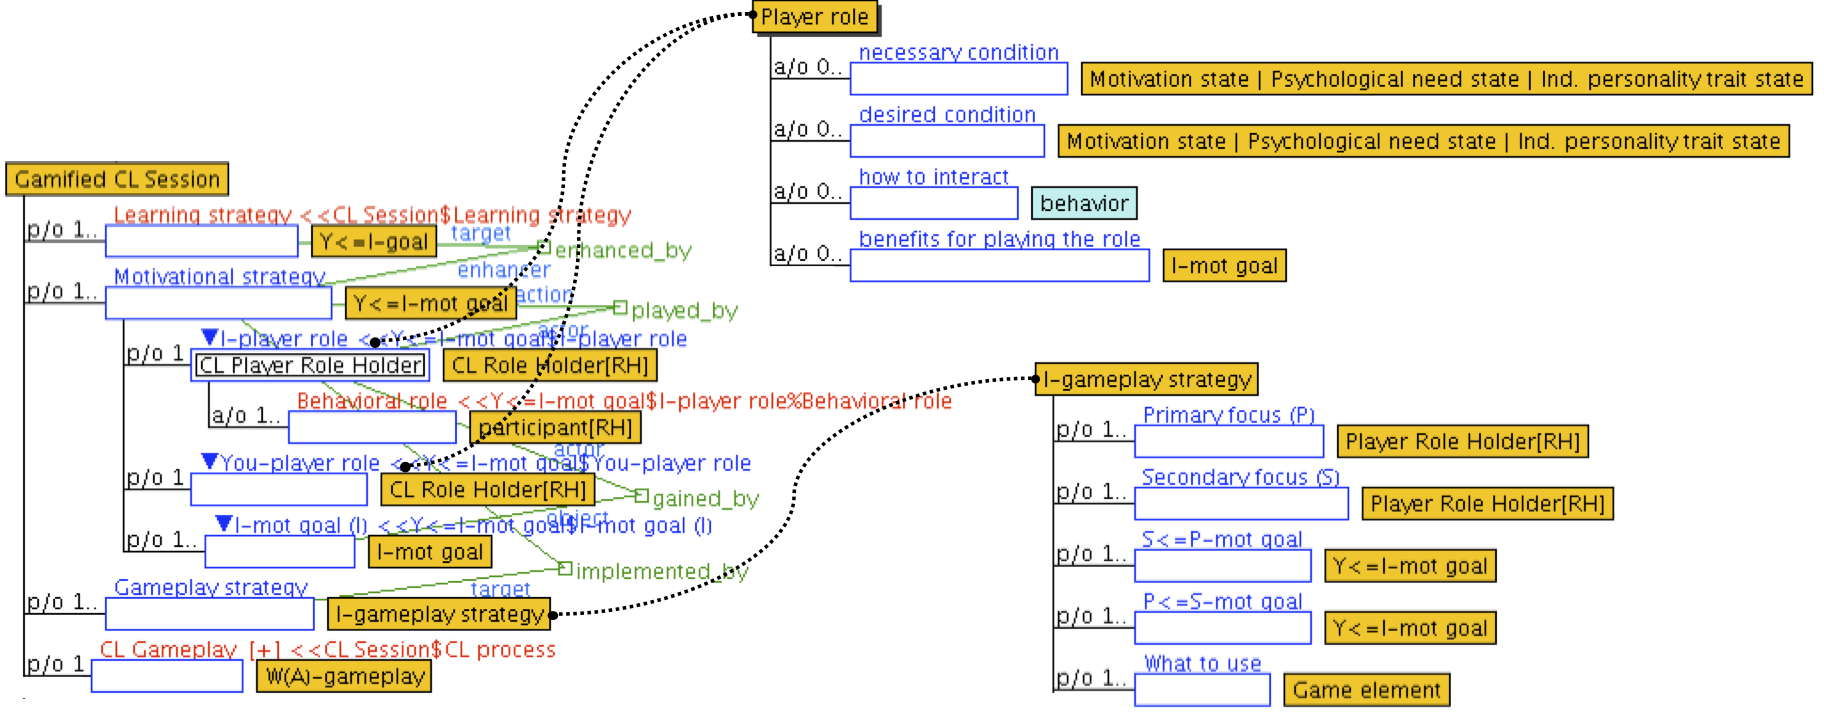
\includegraphics[width=1\textwidth]{images/chap-ontogacles1/ontological-structure-gamified-cl-scenario.png} 
 \fautor
\end{figure}

As was explained in previous subsections, the individual motivational strategy (\emph{Y<=I-mot goal}) describes the guidelines used to enhance the learning strategy employed by the participant in focus (\emph{I}), and the individual gameplay strategy (\emph{I-gameplay strategy}) describes the strategy used to implement the guidelines of individual motivational strategies. Based on these definitions, in the ontological structures to represent a gamified CL scenario (\autoref{fig:ontological-structure-gamified-cl-scenario}), the connection of these elements has been represented by the two relational-concepts: \aspas{\emph{enhanced\_by}} and \aspas{\emph{implemented\_by}.} The relational-concept \aspas{\emph{enhanced\_by}} indicates what individual motivational strategy (\emph{Y<=I-mot goal}) is used to enhance a learning strategy (\emph{Y<=I-goal}), and the relational-concept \aspas{\emph{implemented\_by}} indicates what individual gameplay strategy (\emph{I-gameplay strategy}) is used to implement the guidelines of an individual motivational strategy (\emph{Y<=I-mot goal}).

To illustrate the use of the ontological structures proposed in \autoref{fig:ontological-structure-gamified-cl-scenario}, a gamified CL scenario for participant who plays the Dodecad Socializers has been formalized as shown in \autoref{fig:ontological-structure-gamified-cl-scenario-dodecad-socializers}, where the learning strategies (\emph{Y<=I-goal}) of participants are \emph{enhanced by} the individual motivational strategy \aspas{\emph{Gamifying for Dodecad Socializer}.} According to this motivational strategy:

\begin{citacao}
\aspas{... Socializers are motivated by relatedness. They want to interact with others and create social connections ... Socializers are the ones who want to interact with others. They like to be connected to others. They are interested in parts of the system that help them do this. These are the ones will evangelize your internal social networks. Most motivated by the social connections aspects of relatedness ... Socializer and Networkers will wish to interact with people. Neither will be after anything from people directly. In the case of a networker, their reward comes from being connected; whereas the socialiser's reward is knowing you and interacting with you ...} \citeonline{Marczewski2015d}.
\end{citacao}

Based on these guidelines, the individual motivational strategy \aspas{\emph{Gamifying for Dodecad Socializer}} indicates that a participant who plays the Dodecad Socializer role (\emph{I-player role}) interacts with other socializer (\emph{You-player role}) acting as \emph{Helper} to achieve the \emph{Satisfaction of relatedness} (\emph{I-mot goal}). In this sense, the motivational strategy is \emph{implemented by} a \emph{Social fun gameplay strategy} (\emph{I-gameplay strategy}) in which, to support the communication and cooperation of participants, the game social-status and game social-connections were inferred as necessary game elements to carry out the social fun gameplay strategy. This inference pertains to the author of this thesis, and it consists in that participants who play the socializer role are interesting into help others by looking for social connections and status to satisfy his/her need of relatedness.

\begin{figure}[!htbp]
 \caption[Ontological structures to represent a gamified CL scenario for dodecad socializers]{Ontological structures to represent a \aspas{\emph{Gamified CL Scenario for Dodecad Socializers}}}
 \label{fig:ontological-structure-gamified-cl-scenario-dodecad-socializers}
 \centering
 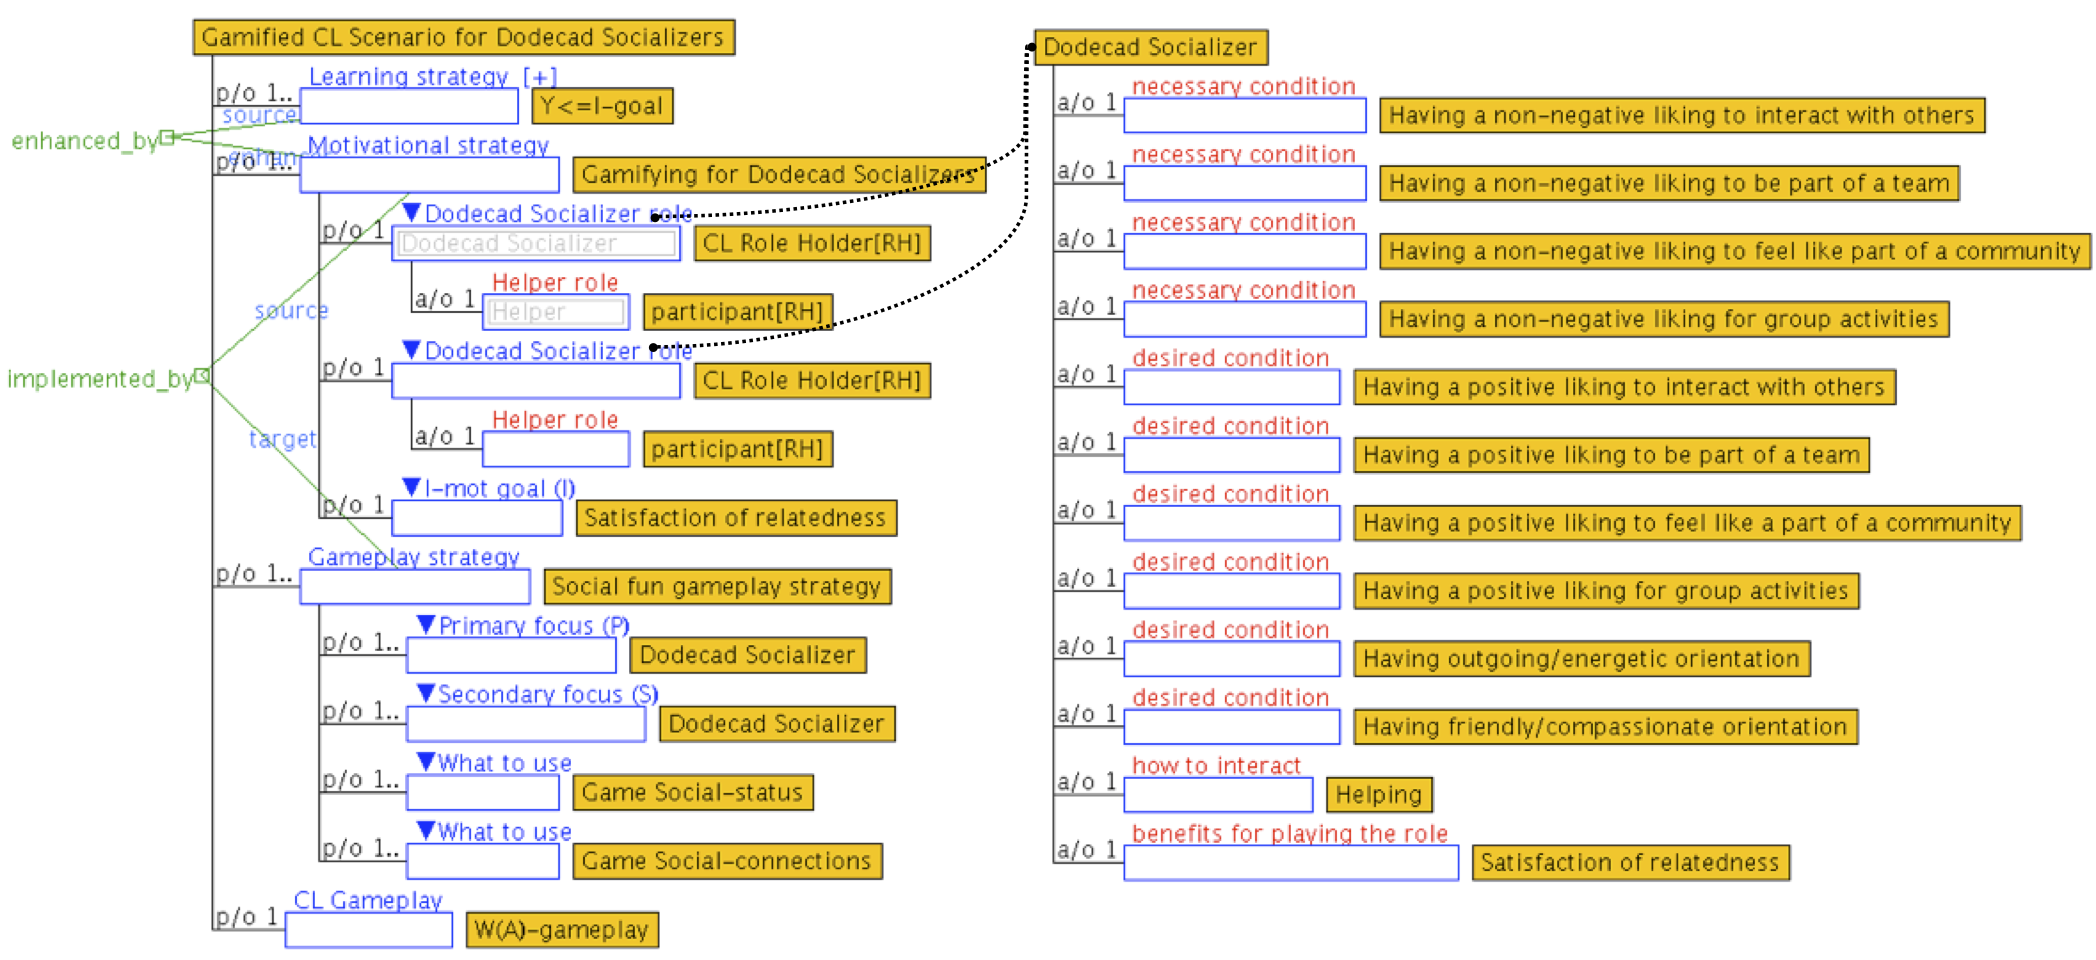
\includegraphics[width=1\textwidth]{images/chap-ontogacles1/ontological-structure-gamified-cl-scenario-dodecad-socializers.png} 
 \fautor
\end{figure}

%%%%%%%%%%%%%%%%%%%%%%%%%%%%%%%%%%%%%%%%%%%%%%%%%%%%

\section[Formalizing an Ontological Model to Personalize the Gamification in CL Scenarios]{Formalizing an Ontological Model to Personalize the Gamification in Collaborative Learning Scenarios}
\label{sec:formalizing-ontological-model}

Through the use of ontological structures presented in the previous section, the author of this thesis expects to facilitate the systematic formalization of gamified CL scenarios based on concepts extracted from player types models and need-based theories of motivation. With this formalization, it is possible to built ontological models to personalize the gamification in CL scenario. These models consist in a set of gamified CL scenarios formally represented as the ontological structures proposed in \autoref{fig:ontological-structure-gamified-cl-scenario}. The building of these structures to define an ontological model comprises the following steps: (1) to identify the player roles that can be assigned for the participants of CL scenario when they are playing a CL role, (2) to identify the restriction and elements of motivational strategies for each pair of identified player roles, and (3) to define individual gameplay strategies for the identified pairs of player roles.

In this section, following these steps, the building of an ontological model to personalize the gamification in CL scenario is detailed in this section. This model has been built to gamify CL scenarios based on the Peer-tutoring theory \cite{Endlsey1980} in which the Dodecad player type model \cite{Marczewski2017,Marczewski2015b} have been used as source of information to formalize this model. 

\subsubsection*{Step (1): Identifying Player Roles for CL Scenarios}  

The identification of player roles to gamify a CL scenario is carried out by analyzing the expected behaviors to be externalized for these roles and the CL roles. Possible counterproductive behaviors indicate what player roles cannot be assigned to a participant when he/she plays the CL role. \autoref{tab:player-roles-in-peer-tutoring-cl-scenarios} shows the result of this step (1) for the CL roles of \aspas{\emph{Peer-Tutor}} and \aspas{\emph{Peer-Tutee}} defined in CL Scenarios based on the Peer-tutoring theory. Counterproductive behaviors of player roles are avoided to not interfere with the expected behaviors of CL roles. Thus, for example, participants who are playing the CL roles of Peer-tutor and Peer-tutee cannot play the \emph{Griefer roles} because they want to negatively affect other users.

\begin{quadro}[htb]
\caption{Dodecad player roles that can be assigned for participants of a Peer-tutoring scenario}
\label{tab:player-roles-in-peer-tutoring-cl-scenarios}
\centering
\scriptsize
\begin{tabular}{|l|c|c|}

\hline%\hline
\multicolumn{1}{|l}{}&
\multicolumn{1}{|c}{\textbf{Peer-Tutor}}&
\multicolumn{1}{|c|}{\textbf{Peer-Tutee}}\tabularnewline
\multicolumn{1}{|l}{}&
\multicolumn{1}{|c}{\footnotesize(explaining)}&
\multicolumn{1}{|c|}{\footnotesize(passive learning)}\tabularnewline
\hline
\hline

\textbf{Achiever}&\multirow{2}{*}{Yes}&\multirow{2}{*}{Yes}\tabularnewline
{\footnotesize(accomplishing, comparing)}& & \tabularnewline
\hline

\textbf{Free-Spirit}&No&No\tabularnewline
{\footnotesize(creating, exploring)}&{\footnotesize(don't want to be restricted)}&{\footnotesize(don't want to be restricted)}\tabularnewline
\hline

\textbf{Socializer}&\multirow{2}{*}{Yes}&\multirow{2}{*}{Yes}\tabularnewline
{\footnotesize(helping)}& & \tabularnewline
\hline

\textbf{Philanthropist}&\multirow{2}{*}{Yes}&\multirow{2}{*}{Yes}\tabularnewline
{\footnotesize(giving, helping, sharing)}& & \tabularnewline
\hline

\textbf{Consumer}&\multirow{2}{*}{Yes}&\multirow{2}{*}{Yes}\tabularnewline
{\footnotesize(accomplishing, comparing)}& & \tabularnewline
\hline

\textbf{Exploiter}&No&No\tabularnewline
{\footnotesize(creating, exploring)}&{\footnotesize(don't want to be restricted)}&{\footnotesize(don't want to be restricted)} \tabularnewline
\hline

\textbf{Networker}&\multirow{2}{*}{Yes}&\multirow{2}{*}{Yes}\tabularnewline
{\footnotesize(helping)}& & \tabularnewline
\hline

\textbf{Self-Seeker}&\multirow{2}{*}{Yes}&\multirow{2}{*}{Yes}\tabularnewline
{\footnotesize(giving, helping, sharing)}& & \tabularnewline
\hline

\textbf{Destroyer}&No&No \tabularnewline
{\footnotesize(hacking)}&{\footnotesize(hacking to ruin experience of others)}&{\footnotesize(hacking to ruin experience of others)}\tabularnewline
\hline

\textbf{Improver}&No&No\tabularnewline
{\footnotesize(hacking, exploring, fixing)}&{\footnotesize(hacking to change the system)}&{\footnotesize(hacking to change the system)}\tabularnewline
\hline

\textbf{Influencer}&No&No \tabularnewline
{\footnotesize(commenting)}&{\footnotesize(requiring changes in the system)}&{\footnotesize(requiring changes in the system)} \tabularnewline
\hline

\textbf{Griefer}&No&No\tabularnewline
{\footnotesize(troublemaking, defying)}&{\footnotesize(negatively affect to others)}&{\footnotesize(negatively affect to others)}\tabularnewline

\hline
\end{tabular}
 \fautor
\end{quadro}


\subsubsection*{Step (2): Identifying Restrictions and Elements of Motivational Strategies}

To identify the restrictions and elements of individual motivational strategies (\emph{Y<=I-mot goal}), guidelines for the pairs of player roles identified in the step (1) are crossed. These guidelines are extracted from the player type models for the building of ontological models to personalize the gamification in CL scenarios. When these guidelines related to a pair of player roles are crossed, counterproductive behaviors are avoided to not interfere with the expected benefits that can be achieved by the participants playing these roles and performing these behaviors. The expected benefits are expressed as individual motivational goals (\emph{I-mot goals}) based on interpretation of these benefits using need-based theories of motivation. 

\autoref{tab:individual-motivational-strategies-in-peer-tutoring-cl-scenarios} shows the result obtained in this step for the definition of individual motivational strategies in the ontological model to personalize the gamification in Peer-tutoring CL scenarios. The rows indicate the player roles (\emph{I-Player role}) for the participant in focus (\emph{I}), and the columns indicate the player roles (\emph{You-Player role}) for the participant (\emph{You}) who interacts with the participant in focus (\emph{I}). The individual gameplay strategies and their elements are indicated in the crossed cells. These strategies were defined from common guidelines for each pair of player roles. Thus, an individual gameplay strategy has been formalized in the ontological model when there are common expected behaviors indicated in the guidelines of player roles \aspas{\emph{I-Player role}} and \aspas{\emph{You-Player role}.}
 

%\setlongtables
\begin{landscape}%{\small
%\begin{longtable}{|l|c|c|c|c|c|c|}
%\caption[Individual motivational strategies identified for the building of an ontological model to personalize the gamification in Peer-tutoring scenarios]{Individual motivational strategies identified for the building of an ontological model to personalize the gamification in Peer-tutoring scenarios}
%\tabularnewline



\begin{quadro}[htb]
\caption{Individual motivational strategies identified for the building of an ontological model to personalize the gamification in Peer-tutoring scenarios}
\label{tab:individual-motivational-strategies-in-peer-tutoring-cl-scenarios}
\centering
\scriptsize
\begin{tabular}{|l|c|c|c|c|c|c|}
\hline%\hline
\multicolumn{1}{|l|}{}&
\multicolumn{1}{c|}{\textbf{Achiever}}&
\multicolumn{1}{c|}{\textbf{Socializer}}&
\multicolumn{1}{c|}{\textbf{Philanthropist}}&
\multicolumn{1}{c|}{\textbf{Consumer}}&
\multicolumn{1}{c|}{\textbf{Networker}}&
\multicolumn{1}{c|}{\textbf{Self-seeker}}\tabularnewline
\multicolumn{1}{|l|}{}&
\multicolumn{1}{c|}{\tiny{(\emph{accomplishing, comparing})}}&
\multicolumn{1}{c|}{\tiny{(\emph{helping})}}&
\multicolumn{1}{c|}{\tiny{(\emph{giving, helping, sharing})}}&
\multicolumn{1}{c|}{\tiny{(\emph{accomplishing, comparing})}}&
\multicolumn{1}{c|}{\tiny{(\emph{helping})}}&
\multicolumn{1}{c|}{\tiny{(\emph{giving, helping, sharing})}}\tabularnewline
\hline
%\endfirsthead\caption[]{\em (continued)} \tabularnewline
\hline
%\multicolumn{1}{|l|}{}&
%\multicolumn{1}{c|}{\textbf{Achiever}}&
%\multicolumn{1}{c|}{\textbf{Socializer}}&
%\multicolumn{1}{c|}{\textbf{Philanthropist}}&
%\multicolumn{1}{c|}{\textbf{Consumer}}&
%\multicolumn{1}{c|}{\textbf{Networker}}&
%\multicolumn{1}{c|}{\textbf{Self-seeker}}\tabularnewline
%\multicolumn{1}{|l|}{}&
%\multicolumn{1}{c|}{\tiny{(\emph{accomplishing, comparing})}}&
%\multicolumn{1}{c|}{\tiny{(\emph{helping})}}&
%\multicolumn{1}{c|}{\tiny{(\emph{giving, helping, sharing})}}&
%\multicolumn{1}{c|}{\tiny{(\emph{accomplishing, comparing})}}&
%\multicolumn{1}{c|}{\tiny{(\emph{helping})}}&
%\multicolumn{1}{c|}{\tiny{(\emph{giving, helping, sharing})}}\tabularnewline
%\hline
%\endhead
%\hline
%\endfoot
%\label{tab:individual-motivational-strategies-in-peer-tutoring-cl-scenarios}
&
\multicolumn{1}{p{3cm}|}{\tiny\emph{Gamifying for Dodecad Achievers}}& & &
\multicolumn{1}{p{3cm}|}{\tiny\emph{Gamifying for Dodecad Achievers and Consumer}}& &  \tabularnewline
{\textbf{Achiever}}&
\multicolumn{1}{p{3cm}|}{\tiny{$\bullet$ Satisfaction of mastery}}& & &
\multicolumn{1}{p{3cm}|}{\tiny{$\bullet$ Satisfaction of mastery}}& & \tabularnewline
{\tiny(\emph{accomplishing, comparing})}&
\multicolumn{1}{p{3cm}|}{}& & &
\multicolumn{1}{p{3cm}|}{\tiny{$\bullet$ Internalization from extrinsic to intrinsic motivation}}& & \tabularnewline
\hline

& &
\multicolumn{1}{p{3cm}|}{\tiny\emph{Gamifying for Dodecad Socializers}}& & &
\multicolumn{1}{p{3cm}|}{\tiny\emph{Gamifying for Dodecad Socializer and Networker}}& \tabularnewline
{\textbf{Socializer}}& &
\multicolumn{1}{p{3cm}|}{\tiny{$\bullet$ Satisfaction of relatedness}}& & &
\multicolumn{1}{p{3cm}|}{\tiny{$\bullet$ Satisfaction of relatedness}}& \tabularnewline
{\tiny(\emph{helping})}& & 
\multicolumn{1}{p{3cm}|}{}& & &
\multicolumn{1}{p{3cm}|}{\tiny{$\bullet$ Internalization from extrinsic to intrinsic motivation}}& \tabularnewline
\hline

\textbf{Philanthropist}& & &
\multicolumn{1}{p{3cm}|}{\tiny\emph{Gamifying for Philanthropists}}& & &
\multicolumn{1}{p{3cm}|}{\tiny\emph{Gamifying for Philanthropist and Self-seeker}}\tabularnewline
{\tiny(\emph{giving, helping, sharing})}& & &
\multicolumn{1}{p{3cm}|}{\tiny{$\bullet$ Satisfaction of purpose}}& & &
\multicolumn{1}{p{3cm}|}{\tiny{$\bullet$ Satisfaction of purpose}}\tabularnewline
& & &
\multicolumn{1}{p{3cm}|}{}& & &
\multicolumn{1}{p{3cm}|}{\tiny{$\bullet$ Internalization from extrinsic to intrinsic motivation}}\tabularnewline
\hline

&
\multicolumn{1}{p{3cm}|}{\tiny\emph{Gamifying for Consumer and Dodecad Achiever}}& & &
\multicolumn{1}{p{3cm}|}{\tiny\emph{Gamifying for Consumers}}& &  \tabularnewline
{\textbf{Consumer}}&
\multicolumn{1}{p{3cm}|}{\tiny{$\bullet$ Satisfaction of mastery}}& & &
\multicolumn{1}{p{3cm}|}{\tiny{$\bullet$ Satisfaction of mastery}}& & \tabularnewline
{\tiny(\emph{accomplishing, comparing})}&
\multicolumn{1}{p{3cm}|}{\tiny{$\bullet$ Internalization from extrinsic to intrinsic motivation}}& & &
\multicolumn{1}{p{3cm}|}{}& & \tabularnewline% \newpage
\hline

& &
\multicolumn{1}{p{3cm}|}{\tiny\emph{Gamifying for Networker and Dodecad Socializer}}& & &
\multicolumn{1}{p{3cm}|}{\tiny\emph{Gamifying for Networkers}}&  \tabularnewline
{\textbf{Networker}}& &
\multicolumn{1}{p{3cm}|}{\tiny{$\bullet$ Satisfaction of relatedness}}& & &
\multicolumn{1}{p{3cm}|}{\tiny{$\bullet$ Satisfaction of relatedness}}& \tabularnewline
{\tiny(\emph{helping})}& & 
\multicolumn{1}{p{3cm}|}{\tiny{$\bullet$ Internalization from extrinsic to intrinsic motivation}}& & &
\multicolumn{1}{p{3cm}|}{}& \tabularnewline
\hline

& & &
\multicolumn{1}{p{3cm}|}{\tiny\emph{Gamifying for Self-seeker and Philanthropist}}& & &
\multicolumn{1}{p{3cm}|}{\tiny\emph{Gamifying for Philanthropists}}\tabularnewline
{\textbf{Self-seeker}}& & &
\multicolumn{1}{p{3cm}|}{\tiny{$\bullet$ Satisfaction of purpose}}& & &
\multicolumn{1}{p{3cm}|}{\tiny{$\bullet$ Satisfaction of purpose}}\tabularnewline
{\tiny(\emph{giving, helping, sharing})}& & &
\multicolumn{1}{p{3cm}|}{\tiny{$\bullet$ Internalization from extrinsic to intrinsic motivation}}& & &
\multicolumn{1}{p{3cm}|}{}\tabularnewline
\hline
%\end{longtable}
%}
\end{tabular}
 \fautor
\end{quadro}
\end{landscape}

To illustrate the identification of restrictions and elements in the individual motivational strategy (\emph{Y<=I-mot goal}), let us see the \aspas{\emph{Gamifying for Dodecad Achiever and Conqueror}} indicated in \autoref{tab:individual-motivational-strategies-in-peer-tutoring-cl-scenarios}, this strategy was identified from the guidelines of Dodecad model in which the behaviors of \emph{accomplishing} and \emph{comparing} are indicated as adequate to motivate achievers and consumers. In this case, the expected benefits to accomplish a goal, and then, compare it against the accomplishments of others is enjoyable for achievers. This benefit is represented as the individual motivational goal \aspas{\emph{Satisfaction of mastery}} (\emph{I-mot goal}) based on the Dan Pink motivation theory \cite{Pink2011}. According to this theory, mastery is a inherit human need that love to get better at stuff enjoying satisfaction from personal achievement and progress.
 
\subsubsection*{Step (3): Defining Individual Gameplay Strategies}

Individual gameplay strategies (\emph{I-gameplay strategy}) are inferred from the individual motivational strategies (\emph{Y<=I-mot goal}) identified in the step (2). Game elements are defined to support the behaviors indicated in the guidelines of individual motivational strategies, and so obtain the expected benefits indicated as individual motivational goal. \autoref{tab:individual-gameplay-strategies-peer-tutoring-cl-scenarios} shows the results of this step for the ontological model to personalize the gamification in Peer-tutoring scenarios.



\begin{quadro}[htb]
\caption{Individual gameplay strategies to gamify Peer-tutoring scenarios}
\label{tab:individual-gameplay-strategies-peer-tutoring-cl-scenarios}
\centering
\small
\begin{tabular}{l|l|l}


%\setlongtables{\small
%\begin{longtable}{l|l|l}
%\caption{Individual gameplay strategies to gamify Peer-tutoring scenarios}
%\tabularnewline
\hline%\hline
\multicolumn{1}{p{4.75cm}}{\centering\textbf{Achievement fun}}&
\multicolumn{1}{|p{4.75cm}|}{\centering\textbf{Social fun}}&
\multicolumn{1}{p{4.75cm}}{\centering\textbf{Facilitated-personal fun}}\tabularnewline
%\hline
%\endfirsthead\caption[]{\em (continued)} \tabularnewline
%\hline
%\multicolumn{1}{p{4.75cm}}{\centering\textbf{Achievement fun}}&
%\multicolumn{1}{|p{4.75cm}|}{\centering\textbf{Social fun}}&
%\multicolumn{1}{p{4.75cm}}{\centering\textbf{Facilitated-personal fun}}\tabularnewline
\hline
%\endhead
\hline
%\endfoot
%\label{tab:individual-gameplay-strategies-peer-tutoring-cl-scenarios}

Primary focus (P):&
Primary focus (P):&
Primary focus (P):\tabularnewline

{\scriptsize$\bullet$ Gamifying for Dodecad Achiever}&
{\scriptsize$\bullet$ Gamifying for Dodecad Socializer}&
{\scriptsize$\bullet$ Gamifying for Philanthropists}\tabularnewline

{\scriptsize$\bullet$ Gamifying for Consumer}&
{\scriptsize$\bullet$ Gamifying for Networker}&
{\scriptsize$\bullet$ Gamifying for Self-seekers}\tabularnewline


Secondary focus (S):&
Secondary focus (S):&
Secondary focus (S):\tabularnewline

{\scriptsize$\bullet$ Gamifying for Consumer}&
{\scriptsize$\bullet$ Gamifying for Networker}&
{\scriptsize$\bullet$ Gamifying for Self-seekers}\tabularnewline

{\scriptsize$\bullet$ Gamifying for Dodecad Achiever}&
{\scriptsize$\bullet$ Gamifying for Dodecad Socializer}&
{\scriptsize$\bullet$ Gamifying for Philanthropists}\tabularnewline
\hline

What to use:&
What to use:&
What to use:\tabularnewline

$\bullet$ Challenges&
$\bullet$ Social-status&
$\bullet$ Meaning/purpose\tabularnewline

$\bullet$ Certificates&
$\bullet$ Point system&
$\bullet$ Access system\tabularnewline

$\bullet$ Levels/progression system&
(\emph{social status})&
$\bullet$ Collect/trade system\tabularnewline

$\bullet$ Point system&
$\bullet$ Physical-reward system&
$\bullet$ Gifting/sharing system\tabularnewline

(\emph{levels/progression})&
(\emph{social status})&
$\bullet$ Point system\tabularnewline

$\bullet$ Physical-reward system&
$\bullet$ Leaderboard system&
(\emph{meaning/purpose})\tabularnewline

(\emph{certificates})&
(\emph{social status})&
$\bullet$ Physical-reward system\tabularnewline

$\bullet$ Leaderboard system&
$\bullet$ Badge system&
(\emph{meaning/purpose})\tabularnewline

(\emph{levels/progression})&
(\emph{social status})&
$\bullet$ Leaderboard system\tabularnewline

$\bullet$ Badge system&
$\bullet$ Virtual-economy system&
(\emph{meaning/purpose})\tabularnewline

(\emph{level/progression})&
$\bullet$ Lottery system&
$\bullet$ Badge system\tabularnewline

$\bullet$ Virtual-economy system&
&
(\emph{meaning/purpose})\tabularnewline

$\bullet$ Lottery system&
&
$\bullet$ Virtual economy system\tabularnewline

&
&
$\bullet$ Lottery system\tabularnewline

\hline
%\end{longtable}
%}
\end{tabular}
 \fautor
\end{quadro}


The individual gameplay strategies indicated in the \autoref{tab:individual-gameplay-strategies-peer-tutoring-cl-scenarios} are:

\begin{itemize}
\item \emph{Achievement fun gameplay strategy}:
is an individual motivational strategy in which the system recognizes achievements through game challenges, certificates and level/progression. To satisfy the mastery need, the system must try to produce in the participants the feel that they are achieving something by performing the interactions indicated by the Peer-tutoring scripts. Thus, the system would use a point system to indicate the levels/progression in the CSCL script, and when the CL scenario is completed as a game challenge, a certificate would be given by a physical-reward system. The leaderboard system would indicate the level/progression of the script. Badges would be obtained by the participants at the end of CL scenario according to the level/progression in the script. Finally, virtual-economy and lottery systems would establish the relation between the levels/progression of the script and the points, ranking in the leaderboard and badges.

\item \emph{Social fun gameplay strategy}:
is an individual motivational strategy in which social status is used to support the feeling of relatedness. In this sense, the system should provide some form of social network/group to indicate and/or create group/collective game elements. Thus, the system would use a points system with a social status system to indicate points gathered by the participant as group. When the CL scenario is completed, the system would give a physical reward for the groups. A leaderboard would provide rankings by groups to indicate the social status of groups. Badges for groups with a social status would be given by the system to groups when the CL scenario is completed. Finally, virtual-economy and lottery systems would establish the relation between the social status of groups in CL scenarios, and the points, physical-rewards, leaderboards, and badges.

\item \emph{Facilitated-personal fun gameplay strategy}:
is an individual motivational strategy in which the excitement from changing the system satisfy the need of purpose. This satisfaction comes from collection and trading valuable things. So when participants help to others, game elements are collected to be converted into something that has a meaningful value. Thus, meaning/purpose should be given to game elements such as points, physical-rewards, leaderboards, and badges, so that the system provides a collect/trade system to change these element for gifting and/or sharable elements (such as elements to customize the avatars, elements to change part of the system).
\end{itemize}

Employing the information of \autoref{tab:individual-gameplay-strategies-peer-tutoring-cl-scenarios}, twelve ontological structures to represent gamified Peer-tutoring scenarios have been formalized in the ontology OntoGaCLeS to define the model to personalize the gamification in Peer-tutoring scenarios based on the Dodecad model \cite{Marczewski2015b}. These structures in the ontological model are: \emph{Gamified Peer Tutoring Scenario for Achievers}, \emph{Gamified Peer Tutoring Scenario for Achiever/Consumer}, \emph{Gamified Peer Tutoring Scenario for Consumer/Achiever}, \emph{Gamified Peer Tutoring Scenario for Consumers}, \emph{Gamified Peer Tutoring Scenario for Socializers}, \emph{Gamified Peer Tutoring Scenario for Socializer/Networker}, \emph{Gamified Peer Tutoring Scenario for Networker/Socializer}, \emph{Gamified Peer Tutoring Scenario for Networkers}, \emph{Gamified Peer Tutoring Scenario for Philanthropists}, \emph{Gamified Peer Tutoring Scenario for Philanthropist/Self-seeker}, \emph{Gamified Peer Tutoring Scenario for Self-seeker/Philanthropist}, and \emph{Gamified Peer Tutoring Scenario for Self-seekers}. 


\begin{figure}[!htbp]
 \caption[Ontological structures to represent a gamified CL scenario for dodecad socializers]{Ontological structure to represent \aspas{\emph{Gamified Peer Tutoring Scenario for Achiever/Consumer}}}
 \label{fig:ontological-structure-gamified-peer-tutoring-scenario-achiever-consumer}
 \centering
  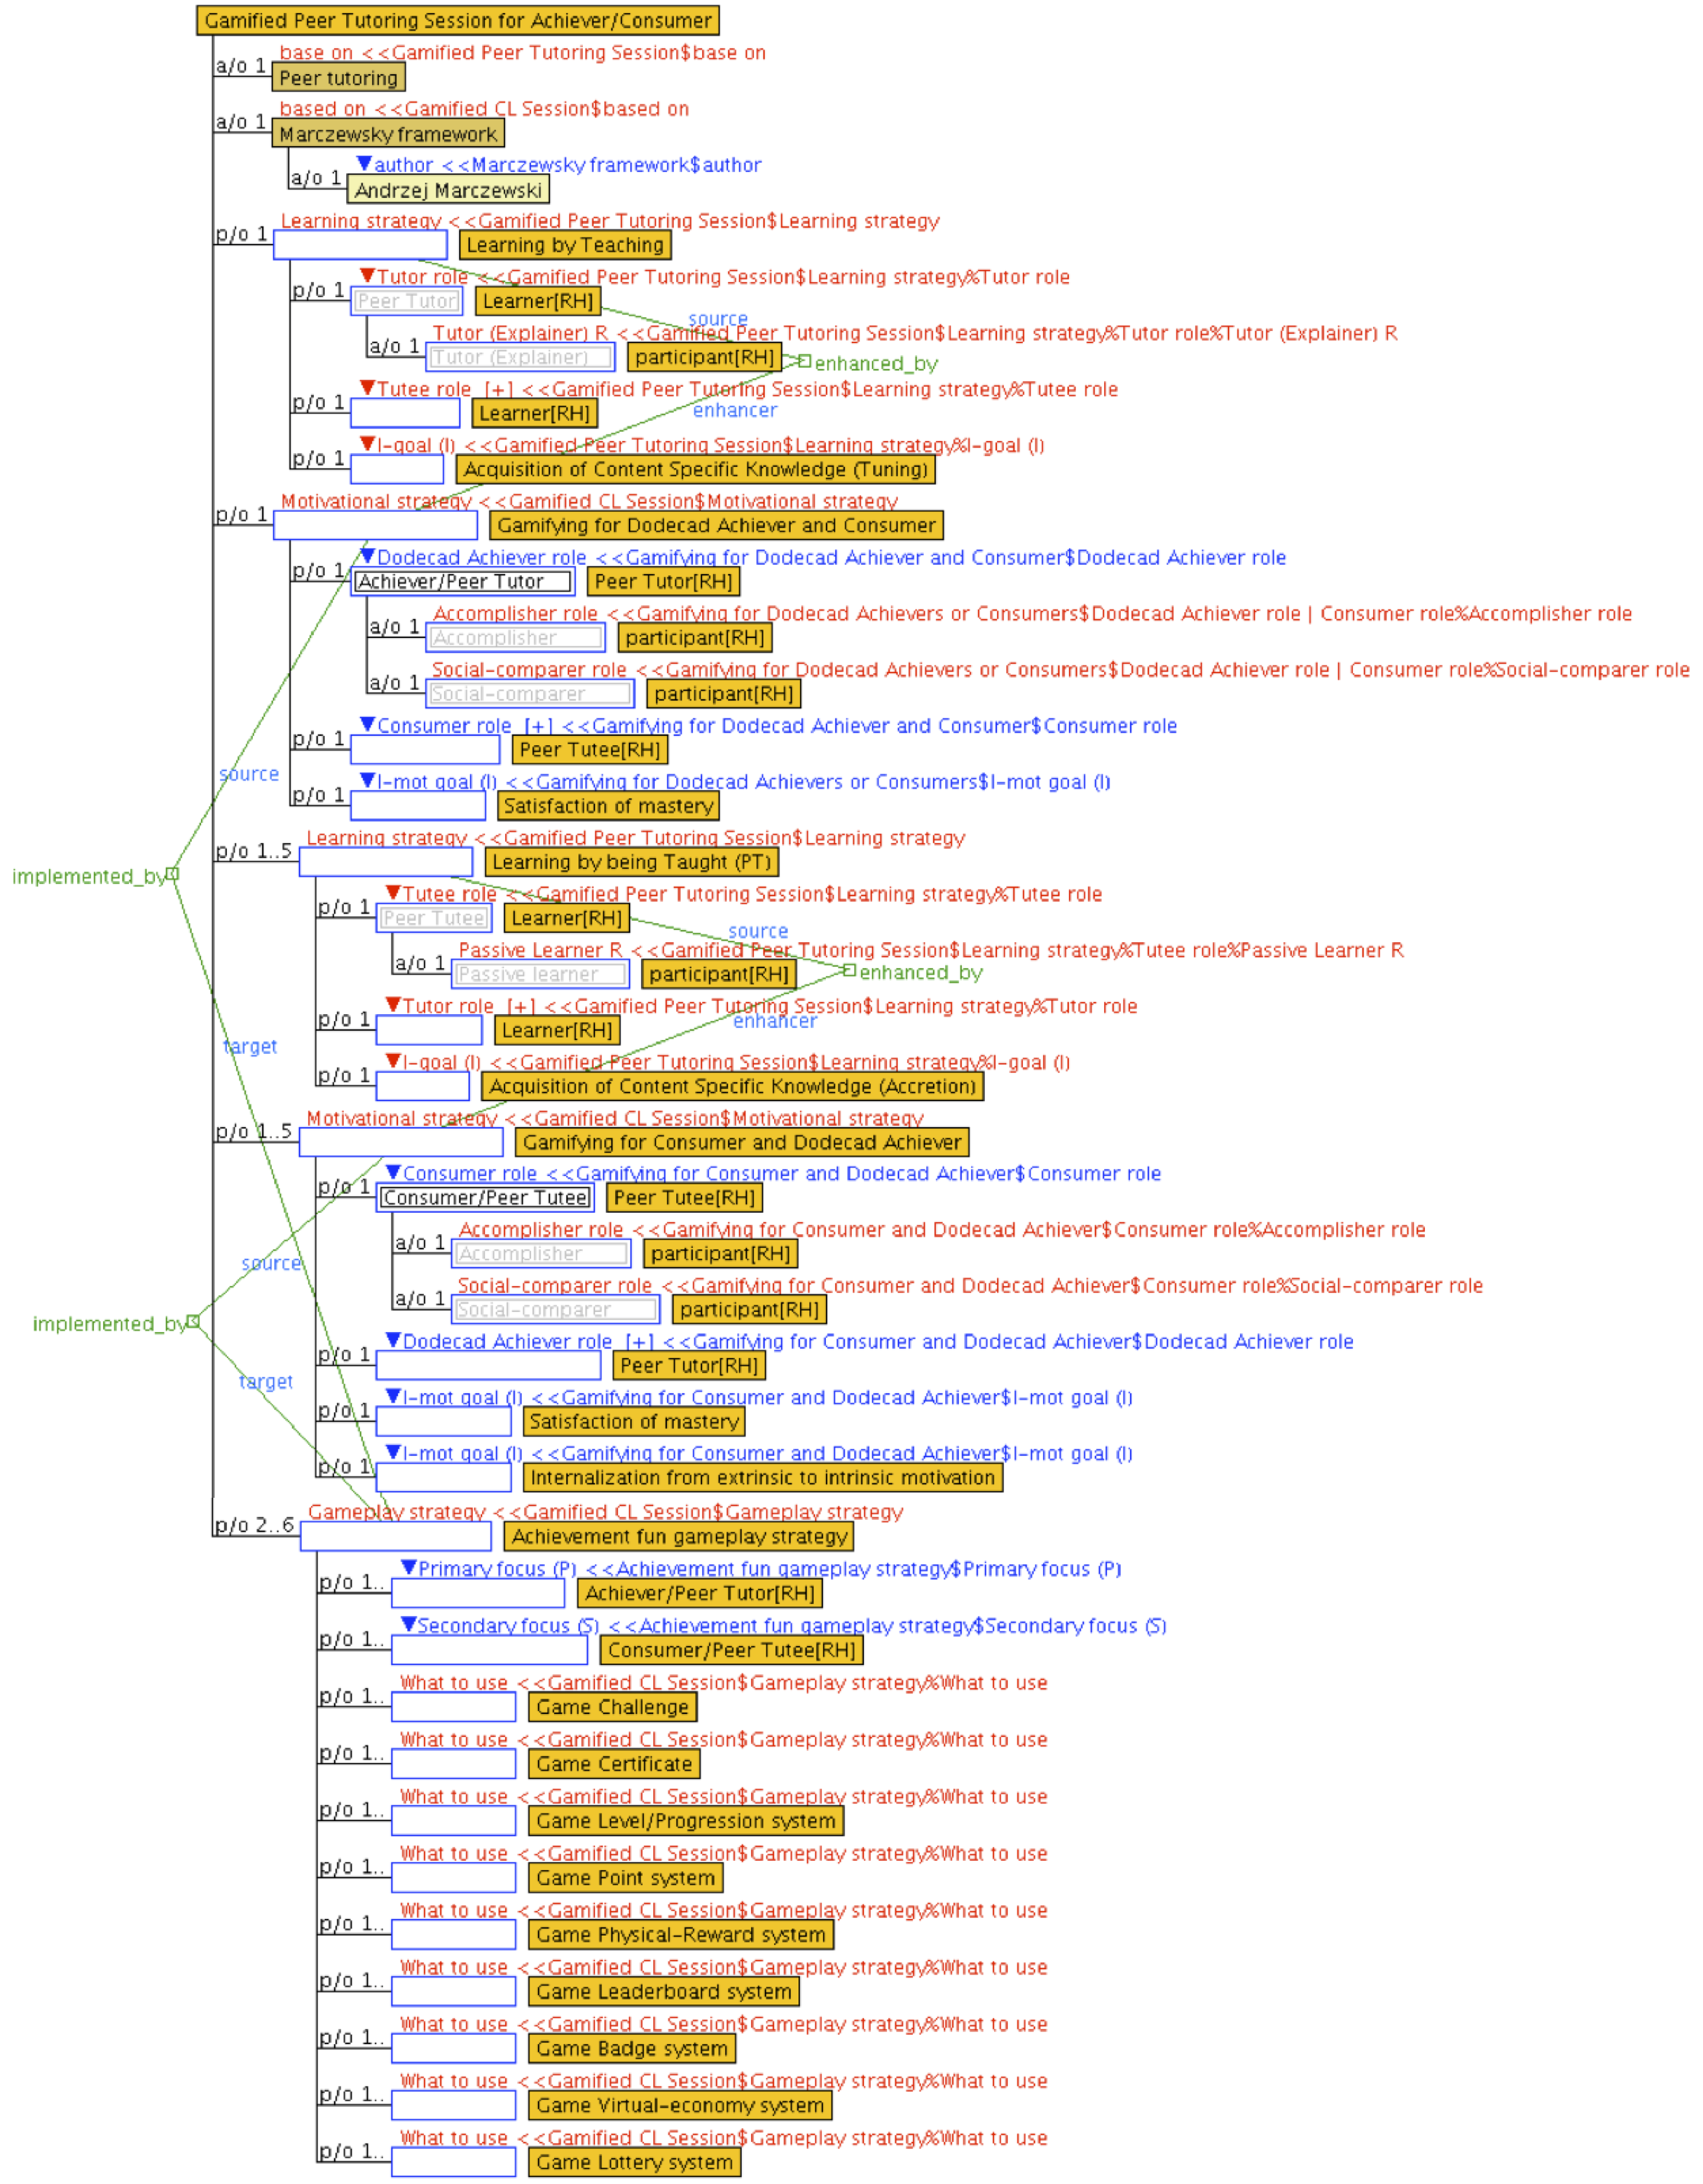
\includegraphics[width=1\textwidth]{images/chap-ontogacles1/ontological-structure-gamified-peer-tutoring-scenario-achiever-consumer.png} 
 \fautor
\end{figure}

\autoref{fig:ontological-structure-gamified-peer-tutoring-scenario-achiever-consumer} shows as example the formalization of \emph{Gamified Peer Tutoring Scenario for Achiever/Consumer} in which the motivational strategy to enhance the learning strategy \aspas{\emph{Learning by Teaching}} is \aspas{\emph{Gamifying for Dodecad Achiever},} and the motivational strategy to enhance the learning strategy \aspas{\emph{Learning by being Taught}} is \aspas{\emph{Gamifiying for Consumer}.} These both motivational strategies are implemented by the gameplay strategy \aspas{\emph{Achievement fun gameplay strategy},} where the participants in the primary focus (P) are holders of \emph{Achiever/Peer Tutor} roles, and the participants in the secondary focus (S) are holders of \emph{Consumer/Peer Tutee} roles. As can be appreciated in the motivational strategy \aspas{\emph{Gamifying for Dodecad Achiever and Consumer},} the potential player for the \emph{Dodecad Achiever role} has been defined as a \emph{Peer Tutor}, and in the motivational strategy \aspas{\emph{Gamifying for Consumer and Dodecad Achiever},} the \emph{Peer Tutee} has been defined as the potential player for the \emph{Consumer role}. 


%%%%%%%%%%%%%%%%%%%%%%%%%%%%%%%%%%%%%%%%%%%%%%%%%%%%

\section{Concluding Remarks}
\label{sec:ontogacles1-concluding-remarks}

In this chapter, concepts extracted from player types models and need-based theories of motivation have been formalized in the ontology OntoGaCLeS to solve the context-dependency related to the participants' individual characteristics and traits when a CL scenario is been gamified to deal with the motivation problem causes by the scripted collaboration. The formalization of these concepts consist in ontological structures to represent individual motivational goals, player roles, motivational strategies, individual gameplay strategies, and gamified CL scenarios.

Through the use of ontological structures proposed in this chapter, it is possible the systematic building of ontology-based models to personalize gamification in CL scenarios based on player types models. This usefulness is demonstrated through an example in which information of Dodecad player type model, is employed to formalize an ontological model to personalize the gamification in Peer-tutoring scenarios. Employing the same formalization, it is possible to obtain ontological models to personalize the gamification in CL scenarios based on other player type models, such as the Yee's model \cite{Yee2006}, Borges' player type model \cite{BorgesMizoguchiDurelliBittencourtIsotani2016}, and BrainHex player type \cite{NackeBatemanMandryk2014}.

With the ontological structures proposed in this chapter, computer-based mechanisms could be built to set player roles and game element for each participant in CL sessions. These mechanisms will use the ontological structures formalized here as a knowledge-base that provide theoretical justification in an algorithm that help the users to gamify CL scenarios. \autoref{chapter:computer-based-mechanisms-procedures} shows a computer-based mechanism developed by the author of this thesis as proof of concept to set player roles for students in CL activities of Moodle platform.


